% !Mode:: "TeX:UTF-8"

\def\usewhat{xelatex} % 定义编译方式 pdflatex, dvipdfmx, or xelatex

\def\xuewei{Course} % 定义学位 Doctor, Master or Bachelor

\def\xueke{Engineering} % 定义学科 Engineering, Science, Management, Arts, Philosophy, Economics, Laws, Education, or History

\newif\ifusexelatex %判断编译环境 
	\def\temp{xelatex}
	\ifx\temp\usewhat
	\usexelatextrue
\fi

\ifusexelatex
	\documentclass[cs4size,openany,twoside,UTF8,normalindentfirst,nofonts]{ctexbook}
\else
	\documentclass[cs4size,openany,twoside,UTF8]{ctexbook}
\fi

% !Mode:: "TeX:UTF-8" 

\makeatletter
\@tempcnta=128
\loop \catcode\@tempcnta=13 \ifnum\@tempcnta<255 \advance \@tempcnta \@ne
\repeat
\makeatother

\newif\ifxueweidoctor %判断论文类型
\newif\ifxueweimaster
\newif\ifxueweibachelor
\newif\ifxueweicourse
\newif\ifNeedEnAbstract
\newif\ifNeedCoverOne
\newif\ifNeedAppendix

\def\temp{Doctor}
\ifx\temp\xuewei
  \xueweidoctortrue
  \xueweimasterfalse
  \xueweibachelorfalse
  \xueweicoursefalse
  \NeedEnAbstracttrue
  \NeedCoverOnetrue
  \NeedAppendixtrue
\fi

\def\temp{Master}
\ifx\temp\xuewei
  \xueweidoctorfalse
  \xueweimastertrue
  \xueweibachelorfalse
  \xueweicoursefalse
  \NeedEnAbstracttrue
  \NeedCoverOnetrue
  \NeedAppendixtrue
\fi

\def\temp{Bachelor}
\ifx\temp\xuewei
  \xueweidoctorfalse  
  \xueweimasterfalse  
  \xueweibachelortrue
  \xueweicoursefalse
  \NeedEnAbstracttrue
  \NeedCoverOnetrue
  \NeedAppendixtrue
\fi

\def\temp{Course}
\ifx\temp\xuewei	
  \xueweidoctorfalse  
  \xueweimasterfalse  
  \xueweibachelorfalse
  \xueweicoursetrue
  \NeedEnAbstractfalse
  \NeedCoverOnefalse
  \NeedAppendixfalse
\fi

\ifxueweidoctor
  \newcommand{\cxuewei}{博士学位}
  \newcommand{\exuewei}{Doctor}
  \newcommand{\exueweier}{Doctoral}
  \newcommand{\xueweishort}{博士}
\fi

\ifxueweimaster
  \newcommand{\cxuewei}{硕士学位}
  \newcommand{\exuewei}{Master}
  \newcommand{\exueweier}{Master's}
  \newcommand{\xueweishort}{硕士}
\fi

\ifxueweibachelor
  \newcommand{\cxuewei}{本科学位}
  \newcommand{\exuewei}{Bachelor}
  \newcommand{\exueweier}{Bachelor's}
  \newcommand{\xueweishort}{学士}
\fi

\ifxueweicourse
  \newcommand{\cxuewei}{课程设计}
  \newcommand{\exuewei}{Course}
  \newcommand{\exueweier}{Course's}
  \newcommand{\xueweishort}{课程}
\fi
    % 类型定义
\ifusexelatex
	% !Mode:: "TeX:UTF-8" 
\xeCJKsetup{AutoFakeBold = false, AutoFakeSlant = false}
\usepackage{tabularx}
\usepackage{graphicx}
\usepackage[a4paper,text={150true mm,224true mm},top=35.5true mm,left=30true mm,head=5true mm,headsep=2.5true mm,foot=8.5true mm]{geometry}
\usepackage{titlesec}               % 控制标题的宏包
\usepackage{titletoc}                   % 控制目录的宏包
\usepackage{fancyhdr}                   % fancyhdr宏包 页眉和页脚的相关定义
\usepackage{color}          % 支持彩色
\usepackage{amsmath}        % AMSLaTeX宏包 用来排出更加漂亮的公式
\usepackage{amssymb}
\usepackage[below]{placeins}%允许上一个section的浮动图形出现在下一个section的开始部分,还提供\FloatBarrier命令,使所有未处理的浮动图形立即被处理
\usepackage{flafter}       % 使得所有浮动体不能被放置在其浮动环境之前,以免浮动体在引述它的文本之前出现.
\usepackage{multirow}       %使用Multirow宏包,使得表格可以合并多个row格
\usepackage{booktabs}       % 表格,横的粗线;\specialrule{1pt}{0pt}{0pt}
\usepackage{longtable}      %支持跨页的表格。
\usepackage[hang]{subfigure}%支持子图 %centerlast 设置最后一行是否居中
\usepackage[subfigure]{ccaption} %支持双语标题
\usepackage[sort&compress,numbers]{natbib}% 支持引用缩写的宏包
\usepackage{enumitem}       %使用enumitem宏包,改变列表项的格式
\usepackage{calc}           %长度可以用+ - * / 进行计算
%\usepackage{txfonts}
\usepackage{fontspec}
\usepackage[amsmath,thmmarks,hyperref]{ntheorem}% 定理类环境宏包,其中 amsmath 选项用来兼容 AMS LaTeX 的宏包

% 生成有书签的pdf及其开关, 该宏包应放在所有宏包的最后, 宏包之间有冲突
\def\atemp{dvipdfmx}\ifx\atemp\usewhat
\usepackage[dvipdfmx,unicode,           %dvi-->pdf 生成书签
            bookmarksnumbered=true,
            bookmarksopen=true,
            colorlinks=false,
            pdfborder={0 0 1},
            citecolor=blue,
            linkcolor=red,
            anchorcolor=green,
            urlcolor=blue,
            breaklinks=true
            ]{hyperref}
\fi

\def\atemp{pdflatex}\ifx\atemp\usewhat
\usepackage{cmap}                       %pdflatex编译时,可以生成可复制、粘贴的中文PDF文档
\usepackage[pdftex,unicode,
            %CJKbookmarks=true,
            bookmarksnumbered=true,
            bookmarksopen=true,
            colorlinks=false,
            pdfborder={0 0 1},
            citecolor=blue,
            linkcolor=red,
            anchorcolor=green,
            urlcolor=blue,
            breaklinks=true
            ]{hyperref}
\fi

\def\atempxetex{xelatex}\ifx\atempxetex\usewhat %\def\atempxetex{xelatex} main.tex中已定义;
\usepackage[xetex,
            bookmarksnumbered=true,
            bookmarksopen=true,
            colorlinks=false,
            pdfborder={0 0 1},
            citecolor=blue,
            linkcolor=red,
            anchorcolor=green,
            urlcolor=blue,
            breaklinks=true,
            naturalnames  %与algorithm2e宏包协调
            ]{hyperref}

\defaultfontfeatures{Mapping=tex-text}
\xeCJKsetemboldenfactor{1}%只对随后定义的CJK字体有效
\setCJKfamilyfont{hei}{SimHei}
\xeCJKsetemboldenfactor{4}
\setCJKfamilyfont{song}{SimSun}
\xeCJKsetemboldenfactor{1}
\setCJKfamilyfont{fs}{FangSong}
\setCJKfamilyfont{kai}{KaiTi}
\setCJKfamilyfont{li}{LiSu}
\setCJKfamilyfont{xw}{STXinwei}
\setCJKmainfont{SimSun}
\setCJKsansfont{SimHei}
\setmainfont{Times New Roman}
\setsansfont{Arial}
\newcommand{\hei}{\CJKfamily{hei}}% 黑体   (Windows自带simhei.ttf)
\newcommand{\song}{\CJKfamily{song}}    % 宋体   (Windows自带simsun.ttf)
\newcommand{\fs}{\CJKfamily{fs}}        % 仿宋体 (Windows自带simfs.ttf)
\newcommand{\kaishu}{\CJKfamily{kai}}      % 楷体   (Windows自带simkai.ttf)
\newcommand{\li}{\CJKfamily{li}}        % 隶书   (Windows自带simli.ttf)
\newcommand{\xw}{\CJKfamily{xw}}        % 隶书   (Windows自带simli.ttf)
\newfontfamily\arial{Arial}
\newfontfamily\timesnewroman{Times New Roman}
\fi

\usepackage[boxed,linesnumbered,algochapter]{algorithm2e}  % 算法的宏包,注意宏包兼容性,先后顺序为float、hyperref、algorithm(2e),否则无法生成算法列表 
\usepackage{xltxtra}
\usepackage{listings}
\lstset{
%basicstyle=\small\ttfamily,
columns=flexible,
breaklines=true
}
 % 引用xe的宏包
\else
	\input{setup/package.tex} % 引用的宏包
\fi

\graphicspath{{figures/}} %定义所有的eps文件在 figures 子目录下

\begin{document}

\ifusexelatex
	% !Mode:: "TeX:UTF-8" 

%\newcommand{\song}{\CJKfamily{song}}    % 宋体   (Windows自带simsun.ttf)
%\newcommand{\hei}{\CJKfamily{hei}}      % 黑体   (Windows自带simhei.ttf)
%\newcommand{\kaishu}{\CJKfamily{kai}}      % 黑体   (Windows自带simhei.ttf)
%\newcommand{\xwei}{\CJKfamily{STXinwei}}

\newcommand{\chuhao}{\fontsize{42pt}{42pt}\selectfont}        % 初号, 单倍行距  本科蛋疼
\newcommand{\xiaochu}{\fontsize{32pt}{32pt}\selectfont}
\newcommand{\yihao}{\fontsize{26pt}{26pt}\selectfont}       % 一号, 1.倍行距
\newcommand{\xiaoyi}{\fontsize{24pt}{24pt}\selectfont}      % 小一, 1.倍行距
\newcommand{\erhao}{\fontsize{22pt}{1.25\baselineskip}\selectfont}       % 二号, 1.倍行距
\newcommand{\xiaoer}{\fontsize{18pt}{18pt}\selectfont}      % 小二, 单倍行距
\newcommand{\sanhao}{\fontsize{16pt}{16pt}\selectfont}      % 三号, 1.倍行距
\newcommand{\xiaosan}{\fontsize{15pt}{15pt}\selectfont}     % 小三, 1.倍行距
\newcommand{\sihao}{\fontsize{14pt}{14pt}\selectfont}       % 四号, 1.0倍行距
\newcommand{\xiaosi}{\fontsize{12pt}{12pt}\selectfont}      % 小四, 1.倍行距
\newcommand{\wuhao}{\fontsize{10.5pt}{10.5pt}\selectfont}   % 五号, 单倍行距
\newcommand{\xiaowu}{\fontsize{9pt}{9pt}\selectfont}        % 小五, 单倍行距


%避免宏包 hyperref 和 arydshln 不兼容带来的目录链接失效的问题。
\def\temp{\relax}
\let\temp\addcontentsline
\gdef\addcontentsline{\phantomsection\temp}

\makeatletter
\gdef\hitempty{}

%重新定义BiChapter命令,可实现标题手动换行,但不影响目录
\def\BiChapter{\relax\@ifnextchar [{\@BiChapter}{\@@BiChapter}}
\def\@BiChapter[#1]#2#3{\chapter[#1]{#2}
    \addcontentsline{toe}{chapter}{\bfseries \xiaosi Chapter \thechapter\hspace{0.5em} #3}}
\def\@@BiChapter#1#2{\chapter{#1}
    \addcontentsline{toe}{chapter}{\bfseries \xiaosi Chapter \thechapter\hspace{0.5em}{\boldmath #2}}}

\newcommand{\BiSection}[2]
{   \section{#1}
    \addcontentsline{toe}{section}{\protect\numberline{\csname thesection\endcsname}#2}
}

\newcommand{\BiSubsection}[2]
{    \subsection{#1}
    \addcontentsline{toe}{subsection}{\protect\numberline{\csname thesubsection\endcsname}#2}
}

\newcommand{\BiSubsubsection}[2]
{    \subsubsection{#1}
    \addcontentsline{toe}{subsubsection}{\protect\numberline{\csname thesubsubsection\endcsname}#2}
}

\newcommand{\BiAppendixChapter}[2] % 该附录命令适用于发表文章,简历等
{\phantomsection
\markboth{#1}{#1}
\addcontentsline{toc}{chapter}{\xiaosi #1}
\addcontentsline{toe}{chapter}{\bfseries \xiaosi #2}  \chapter*{#1}
}

\newcommand{\BiAppChapter}[2]    % 该附录命令适用于有章节的完整附录
{\phantomsection 
 \chapter{#1}
 \addcontentsline{toe}{chapter}{\bfseries \xiaosi Appendix \thechapter~~#2}
}

\renewcommand{\thefigure}{\arabic{chapter}-\arabic{figure}}%使图编号为 7-1 的格式 %\protect{~}
\renewcommand{\thesubfigure}{\alph{subfigure})}%使子图编号为 a)的格式
\renewcommand{\p@subfigure}{\thefigure~} %使子图引用为 7-1 a) 的格式,母图编号和子图编号之间用~加一个空格
\renewcommand{\thetable}{\arabic{chapter}-\arabic{table}}%使表编号为 7-1 的格式
\renewcommand{\theequation}{\arabic{chapter}-\arabic{equation}}%使公式编号为 7-1 的格式

\newcommand{\algoenname}{Algo.} %算法英文标题
\newfloatlist[chapter]{algoen}{aen}{\listalgoenname}{\algoenname}
\newfixedcaption{\algoencaption}{algoen}
\renewcommand{\thealgoen}{\thechapter-\arabic{algocf}}
\renewcommand{\@cftmakeaentitle}{\chapter*{\listalgoenname\@mkboth{\bfseries\listalgoenname}{\bfseries\listalgoenname}}}

\renewcommand{\algorithmcfname}{算法}
\setlength\AlCapSkip{1.2ex}
\SetAlgoSkip{1pt}
\renewcommand{\algocf@captiontext}[2]{\wuhao#1\algocf@typo ~ \AlCapFnt{}#2} % text of caption
\expandafter\ifx\csname algocf@within\endcsname\relax% if \algocf@within doesn't exist
\renewcommand\thealgocf{\@arabic\c@algocf} % and the way it is printed
\else%                                    else
\renewcommand\thealgocf{\csname the\algocf@within\endcsname-\@arabic\c@algocf}
\fi
\renewcommand{\algocf@makecaption}[2]{%中英文双标题一定多于一行,因此去掉单行时的判断,并将\parbox中标题设置为居中
  \addtolength{\hsize}{\algomargin}%
  \sbox\@tempboxa{\algocf@captiontext{#1}{#2}}%
    \hskip .5\algomargin%
    \parbox[t]{\hsize}{\centering\algocf@captiontext{#1}{#2}}% 
  \addtolength{\hsize}{-\algomargin}%
}
\newcommand{\AlgoBiCaption}[2]{%直接取出自定义的中英文标题条目加入到真正的\caption 中  
   \caption[#1]{\protect\setlength{\baselineskip}{1.5em}#1 \protect \\ Algo. \thealgocf~~ #2} % \algoencaption{#2}   
   \addcontentsline{aen}{algoen}{\protect\numberline{\thealgoen}{#2}}
   }

\makeatother

%定义 学科 学位
\def \xuekeEngineering {Engineering}
\def \xuekeScience {Science}
\def \xuekeManagement {Management}
\def \xuekeArts {Arts}
\def \xuekePhilosophy {Philosophy}
\def \xuekeEconomics {Economics}
\def \xuekeLaws {Laws}
\def \xuekeEducation {Education}
\def \xuekeHistory {History}


\ifx \xueke \xuekeEngineering
\newcommand{\cxueke}{工学}
\newcommand{\exueke}{Engineering}
\fi

\ifx \xueke \xuekeScience
\newcommand{\cxueke}{理学}
\newcommand{\exueke}{Science}
\fi

\ifx \xueke \xuekeManagement
\newcommand{\cxueke}{管理学}
\newcommand{\exueke}{Management}
\fi

\ifx \xueke \xuekeArts
\newcommand{\cxueke}{文学}
\newcommand{\exueke}{Arts}
\fi 

\ifx \xueke \xuekePhilosophy
\newcommand{\cxueke}{哲学}
\newcommand{\exueke}{Philosophy}
\fi 

\ifx \xueke \xuekeEconomics
\newcommand{\cxueke}{经济学}
\newcommand{\exueke}{Economics}
\fi 

\ifx \xueke \xuekeLaws
\newcommand{\cxueke}{法学}
\newcommand{\exueke}{Laws}
\fi 

\ifx \xueke \xuekeEducation
\newcommand{\cxueke}{教育学}
\newcommand{\exueke}{Education}
\fi 

\ifx \xueke \xuekeHistory
\newcommand{\cxueke}{历史学}
\newcommand{\exueke}{History}
\fi 
 % 文本xe格式定义
\else
	\input{setup/Definition} % 文本格式定义
\fi


\frontmatter
\ifusexelatex
	\ifxueweibachelor
		% !Mode:: "TeX:UTF-8" 

\theoremstyle{plain}
\theorembodyfont{\song\rmfamily}
\theoremheaderfont{\hei\rmfamily}
\newtheorem{definition}{\hei 定义}[chapter]
\newtheorem{example}{\hei 例}[chapter]
\newtheorem{algo}{\hei 算法}[chapter]
\newtheorem{theorem}{\hei 定理}[chapter]
\newtheorem{axiom}{\hei 公理}[chapter]
\newtheorem{proposition}{\hei 命题}[chapter]
\newtheorem{lemma}{\hei 引理}[chapter]
\newtheorem{corollary}{\hei 推论}[chapter]
\newtheorem{remark}{\hei 注解}[chapter]
\newenvironment{proof}{\noindent{\hei 证明:}}{\hfill $ \square $ \vskip 4mm}
\theoremsymbol{$\square$}
\setlength{\theorempreskipamount}{0pt}
\setlength{\theorempostskipamount}{-2pt}

\allowdisplaybreaks[4]

%\CJKcaption{gb_452} 
%\CJKtilde
\setlength{\parindent}{2em}

\arraycolsep=1.6pt

\renewcommand\contentsname{\hei 目~~~~录}

\CTEXsetup[number={\arabic{chapter}}]{chapter}
\renewcommand\chaptername{第~\thechapter~章}

\setcounter{secnumdepth}{4} \setcounter{tocdepth}{2}


\titleformat{\chapter}{\center\xiaoer\hei}{\chaptertitlename}{0.5em}{}
\titlespacing{\chapter}{0pt}{-5.5mm}{8mm}
\titleformat{\section}{\xiaosan\hei}{\thesection}{0.5em}{}
\titlespacing{\section}{0pt}{4.5mm}{4.5mm}
\titleformat{\subsection}{\sihao\hei}{\thesubsection}{0.5em}{}
\titlespacing{\subsection}{0pt}{4mm}{4mm}
\titleformat{\subsubsection}{\xiaosi\hei}{\thesubsubsection}{0.5em}{}
\titlespacing{\subsubsection}{0pt}{0pt}{0pt}

\titlecontents{chapter}[3.8em]{\hspace{-3.8em}\hei}{\thecontentslabel~~}{}{\titlerule*[4pt]{.}\contentspage}
\dottedcontents{section}[32pt]{}{21pt}{0.3pc}
\dottedcontents{subsection}[53pt]{}{30pt}{0.3pc}


% 按工大标准, 缩小目录中各级标题之间的缩进,使它们相隔一个字符距离,也就是12pt
\makeatletter
\renewcommand*\l@chapter{\@dottedtocline{0}{0em}{5em}}%控制英文目录: 细点\@dottedtocline  粗点\@dottedtoclinebold
\renewcommand*\l@section{\@dottedtocline{1}{1em}{1.8em}}
\renewcommand*\l@subsection{\@dottedtocline{2}{2em}{2.5em}}


% 定义页眉和页脚
\newcommand{\makeheadrule}{
\rule[7pt]{\textwidth}{0.75pt} \\[-23pt]
\rule{\textwidth}{2.25pt}}
\renewcommand{\headrule}{
    {\if@fancyplain\let\headrulewidth\plainheadrulewidth\fi
     \makeheadrule}}
\pagestyle{fancyplain}

%去掉章节标题中的数字
%%不要注销这一行,否则页眉会变成:“第1章1  绪论”样式
\renewcommand{\chaptermark}[1]{\markboth{\chaptertitlename~\ #1}{}}
\fancyhf{}

%在book文件类别下,\leftmark自动存录各章之章名,\rightmark记录节标题
%% 页眉字号 工大要求 小五
%根据单双面打印设置不同的页眉;

\ifxueweidoctor
	\fancyhead[CO]{\song \xiaowu\leftmark}
  	\fancyhead[CE]{\song \xiaowu 哈尔滨工业大学\cxueke\cxuewei 论文 }%
  	\fancyfoot[C,C]{\xiaowu -~\thepage~-}
\fi

\ifxueweimaster  
	\fancyhead[CO]{\song \xiaowu 哈尔滨工业大学\cxueke\cxuewei 论文}
    \fancyhead[CE]{\song \xiaowu 哈尔滨工业大学\cxueke\cxuewei 论文}%
    \fancyfoot[C,C]{\xiaowu -~\thepage~-}
\fi

\ifxueweibachelor  	
    \fancyhead[CO]{\song \xiaowu 哈尔滨工业大学\cxueke\cxuewei 论文}
	\fancyhead[CE]{\song \xiaowu 哈尔滨工业大学\cxueke\cxuewei 论文}%
   	\fancyfoot[C,C]{\xiaowu -~\thepage~-}
\fi

\ifxueweicourse
	\fancyhead[CO]{\song \xiaowu 哈尔滨工业大学 \cxuewei(论文)}
   	\fancyhead[CE]{\song \xiaowu 哈尔滨工业大学 \cxuewei(论文)}%
   	\fancyfoot[C,C]{\xiaowu -~\thepage~-}
\fi

\renewcommand\frontmatter{\cleardoublepage
  \@mainmatterfalse
  \pagenumbering{Roman}}

% 调整罗列环境的布局
\setitemize{leftmargin=0em,itemsep=0em,partopsep=0em,parsep=0em,topsep=0em,itemindent=3em}
\setenumerate{leftmargin=0em,itemsep=0em,partopsep=0em,parsep=0em,topsep=0em,itemindent=3.5em}

\newcommand{\citeup}[1]{\textsuperscript{\cite{#1}}}

% 定制浮动图形和表格标题样式
\captionnamefont{\wuhao}
\captiontitlefont{\wuhao}
\captiondelim{~~}
%\captionstyle{\hang}
\hangcaption
\renewcommand{\subcapsize}{\wuhao}
\setlength{\abovecaptionskip}{0pt}
\setlength{\belowcaptionskip}{0pt}

% 自定义项目列表标签及格式 \begin{publist} 列表项 \end{publist}
\newcounter{pubctr} %自定义新计数器
\newenvironment{publist}{%%%%%定义新环境
\begin{list}{[\arabic{pubctr}]} %%标签格式
    {
     \usecounter{pubctr}
     \setlength{\leftmargin}{1.7em}     % 左边界 \leftmargin =\itemindent + \labelwidth + \labelsep
     \setlength{\itemindent}{0em}     % 标号缩进量
     \setlength{\labelsep}{0.5em}       % 标号和列表项之间的距离,默认0.5em
     \setlength{\rightmargin}{0em}    % 右边界
     \setlength{\topsep}{0ex}         % 列表到上下文的垂直距离
     \setlength{\parsep}{0ex}         % 段落间距
     \setlength{\itemsep}{0ex}        % 标签间距
     \setlength{\listparindent}{0pt} % 段落缩进量
    }}
{\end{list}}%%%%%

% 默认字体
\renewcommand\normalsize{
  \@setfontsize\normalsize{12pt}{12pt}
  \setlength\abovedisplayskip{4pt}
  \setlength\abovedisplayshortskip{4pt}
  \setlength\belowdisplayskip{\abovedisplayskip}
  \setlength\belowdisplayshortskip{\abovedisplayshortskip}
  \let\@listi\@listI}
  
% 设置行距和段落间垂直距离
\def\defaultfont{\renewcommand{\baselinestretch}{1.62}\normalsize\selectfont}
\renewcommand{\CJKglue}{\hskip 0.56pt plus 0.08\baselineskip} 
%加大字间距,使每行34个字,若要使得每行33个字,则将0.56pt替换为0.96pt。
\predisplaypenalty=0  %公式之前可以换页,公式出现在页面顶部

% 封面、摘要、版权、致谢格式定义
\def\ctitle#1{\def\@ctitle{#1}}\def\@ctitle{}
\def\ctitleone#1{\def\@ctitleone{#1}}\def\@ctitleone{}
\def\ctitletwo#1{\def\@ctitletwo{#1}}\def\@ctitletwo{}
\def\cdegree#1{\def\@cdegree{#1}}\def\@cdegree{}
\def\caffil#1{\def\@caffil{#1}}\def\@caffil{}
\def\csubject#1{\def\@csubject{#1}}\def\@csubject{}
\def\cauthor#1{\def\@cauthor{#1}}\def\@cauthor{}
\def\cstuid#1{\def\@cstuid{#1}}\def\@cstuid{} % 本科蛋疼学号
\def\csupervisor#1{\def\@csupervisor{#1}}\def\@csupervisor{}
\def\cassosupervisor#1{\def\@cassosupervisor{{\hei 副 \hfill 导 \hfill 师} & #1\\}}\def\@cassosupervisor{}
\def\ccosupervisor#1{\def\@ccosupervisor{{\hei 联 \hfill 合\hfill 导 \hfill 师} & #1\\}}\def\@ccosupervisor{}
\def\cdate#1{\def\@cdate{#1}}\def\@cdate{}
\long\def\cabstract#1{\long\def\@cabstract{#1}}\long\def\@cabstract{}
\def\ckeywords#1{\def\@ckeywords{#1}}\def\@ckeywords{}

\def\etitle#1{\def\@etitle{#1}}\def\@etitle{}
\def\edegree#1{\def\@edegree{#1}}\def\@edegree{}
\def\eaffil#1{\def\@eaffil{#1}}\def\@eaffil{}
\def\esubject#1{\def\@esubject{#1}}\def\@esubject{}
\def\eauthor#1{\def\@eauthor{#1}}\def\@eauthor{}
\def\esupervisor#1{\def\@esupervisor{#1}}\def\@esupervisor{}
\def\eassosupervisor#1{\def\@eassosupervisor{\textbf{Associate Supervisor:} & #1\\}}\def\@eassosupervisor{}
\def\ecosupervisor#1{\def\@ecosupervisor{\textbf{Co Supervisor:} & #1\\}}\def\@ecosupervisor{}
\def\edate#1{\def\@edate{#1}}\def\@edate{}
\long\def\eabstract#1{\long\def\@eabstract{#1}}\long\def\@eabstract{}
\long\def\NotationList#1{\long\def\@NotationList{#1}}\long\def\@NotationList{}
\def\ekeywords#1{\def\@ekeywords{#1}}\def\@ekeywords{}
\def\natclassifiedindex#1{\def\@natclassifiedindex{#1}}\def\@natclassifiedindex{}
\def\internatclassifiedindex#1{\def\@internatclassifiedindex{#1}}\def\@internatclassifiedindex{}
\def\statesecrets#1{\def\@statesecrets{#1}}\def\@statesecrets{}

% 定义封面
\def\makecover{
    \begin{titlepage}
      % 封面一
      \ifNeedEnAbstract
      \vspace*{0.8cm}
      \begin{center}
     
    \parbox[t][3.4cm][t]{\textwidth}{
    \begin{center}\erhao\hei\@ctitle\end{center} }
    
    \parbox[t][9.4cm][t]{\textwidth}{
        \begin{center}\xiaoer\song\textbf{\@cauthor}\end{center}}
  

            {\hei \xiaosi
            	\begin{tabularx}{6.768cm}{r@{:}c}
            		院\hfill(系) & \@caffil\\
            		学\quad \quad 号 & \@cstuid
            	\end{tabularx}}
 			{\hei \xiaosi
 				\begin{tabularx}{6.768cm}{r@{:}c}
 					专\hfill 业 & \@csubject\\
 					任课教师 & \@csupervisor
 				\end{tabularx}}


    \vspace*{3.0cm}
    
    {\song\xiaosi\textbf{\@cdate}}

    \end{center}

    \newpage
    \fi
    %内封
    \thispagestyle{empty}

\begin{center}

	\vspace*{0.6cm}
	
   % \parbox[t][3.2cm][t]{\textwidth}{\begin{center} \end{center} }
    
    \begin{figure}[htbp]
   	\centering
   	
\includegraphics[scale=0.38]{logo.jpg}
   	\end{figure}
   	
   	\vspace*{0.75cm}
   	
   	{\xw\xiaochu\textbf{概率论与数理统计(小论文)}} % 字体等待替换中
   	
   	 %教务处去死吧,不知道华文新魏是付费的吗你妹,呵呵!先上图!
%   	\begin{figure}[htbp]
%	\centering
%	
\includegraphics[scale=0.25]{hehejwc.png}
%	\end{figure}
	
    \vspace*{1.7cm}
    
	\parbox[t][14.2cm][b]{\textwidth}
     {\xiaosan
    \begin{center} \renewcommand{\arraystretch}{2.5} \hei
    \begin{tabular}{l@{\ \  }c}
    {\hei\xiaoer  题\hfill 目}                  & \underline{\makebox[6.1cm]{\xiaoer \@ctitleone}}\\
%    &  \underline{\makebox[6.1cm]{\xiaoer \@ctitletwo}}\\
%	& \\
    {\hei 专\hfill 业}                  & \underline{\makebox[6.1cm]{\@csubject}}\\
    {\hei 学\hfill 号}                  & \underline{\makebox[6.1cm]{\@cstuid}}\\
    {\hei 学\hfill 生}                  & \underline{\makebox[6.1cm]{\@cauthor}}\\
    {\hei 任\hfill 课\hfill 教\hfill 师} & \underline{\makebox[6.1cm]{\@csupervisor}}\\
    {\hei 日\hfill 期} & \underline{\makebox[6.1cm]{\@cdate}}
    \end{tabular} \renewcommand{\arraystretch}{1}
    \end{center} }
\end{center}

    \end{titlepage}

%%%%%%%%%%%%%%%%%%%   Abstract and keywords  %%%%%%%%%%%%%%%%%%%%%%%
\clearpage

\BiAppendixChapter{摘\quad 要}{Abstract (In Chinese)}

\setcounter{page}{1}
\song\defaultfont
\@cabstract
\vspace{\baselineskip}

\hangafter=1\hangindent=51pt\noindent
{\hei 关键词}:\@ckeywords

%%%%%%%%%%%%%%%%%%%   English Abstract  %%%%%%%%%%%%%%%%%%%%%%%%%%%%%%
\ifNeedCoverOne

\clearpage

\phantomsection
\markboth{Abstract}{Abstract}
\addcontentsline{toc}{chapter}{\xiaosi ABSTRACT}
\addcontentsline{toe}{chapter}{\bfseries \xiaosi Abstract (In English)}  
\addtocontents{toc}{\vspace{\baselineskip}}
\addtocontents{toe}{\vspace{\baselineskip}}
\chapter*{\bf Abstract}
\@eabstract
\vspace{\baselineskip}

\hangafter=1\hangindent=60pt\noindent
{\textbf{Keywords:}}  \@ekeywords

\fi
}


%%%%%%%%%%%%%%%%%%%%%%%%%%%%%%%%%%%%%%%%%%%%%%%%%%%%%%%%%%%%%%%
% 英文目录格式
\def\@dotsep{0.75}           % 定义英文目录的点间距
\setlength\leftmargini {0pt}
\setlength\leftmarginii {0pt}
\setlength\leftmarginiii {0pt}
\setlength\leftmarginiv {0pt}
\setlength\leftmarginv {0pt}
\setlength\leftmarginvi {0pt}

\def\engcontentsname{\bfseries Contents}
\newcommand\tableofengcontents{
   \pdfbookmark[0]{Contents}{econtent}
     \@restonecolfalse
   \chapter*{\engcontentsname  %chapter*上移一行,避免在toc中出现。
       \@mkboth{%
          \engcontentsname}{\engcontentsname}}
   \@starttoc{toe}%
   \if@restonecol\twocolumn\fi
   }

\urlstyle{same}  %论文中引用的网址的字体默认与正文中字体不一致,这里修正为一致的。

\renewcommand\endtable{\vspace{-4mm}\end@float}

\makeatother

% magic282 added some cmds here
\renewcommand{\subcapsize}{\centering\song\wuhao} % 为了使子图的长标题居中
 % 本科xe蛋疼格式
	\fi
	\ifxueweimaster
		% !Mode:: "TeX:UTF-8" 

\theoremstyle{plain}
\theorembodyfont{\song\rmfamily}
\theoremheaderfont{\hei\rmfamily}
\newtheorem{definition}{\hei 定义}[chapter]
\newtheorem{example}{\hei 例}[chapter]
\newtheorem{algo}{\hei 算法}[chapter]
\newtheorem{theorem}{\hei 定理}[chapter]
\newtheorem{axiom}{\hei 公理}[chapter]
\newtheorem{proposition}{\hei 命题}[chapter]
\newtheorem{lemma}{\hei 引理}[chapter]
\newtheorem{corollary}{\hei 推论}[chapter]
\newtheorem{remark}{\hei 注解}[chapter]
\newenvironment{proof}{\noindent{\hei 证明:}}{\hfill $ \square $ \vskip 4mm}
\theoremsymbol{$\square$}
\setlength{\theorempreskipamount}{0pt}
\setlength{\theorempostskipamount}{-2pt}

\allowdisplaybreaks[4]

%\CJKcaption {gb_452} 
%\CJKtilde
\setlength{\parindent}{2em}

\arraycolsep=1.6pt

\renewcommand\contentsname{\hei 目~~~~录}

\CTEXsetup[number={\arabic{chapter}}]{chapter}
\renewcommand\chaptername{第~\thechapter~章}

%\CTEXsetup[name={第,章}]{chapter}
\setcounter{secnumdepth}{4} \setcounter{tocdepth}{2}


\titleformat{\chapter}{\center\xiaoer\hei}{\chaptertitlename}{0.5em}{}
\titlespacing{\chapter}{0pt}{-5.5mm}{8mm}
\titleformat{\section}{\xiaosan\hei}{\thesection}{0.5em}{}
\titlespacing{\section}{0pt}{4.5mm}{4.5mm}
\titleformat{\subsection}{\sihao\hei}{\thesubsection}{0.5em}{}
\titlespacing{\subsection}{0pt}{4mm}{4mm}
\titleformat{\subsubsection}{\xiaosi\hei}{\thesubsubsection}{0.5em}{}
\titlespacing{\subsubsection}{0pt}{0pt}{0pt}

\titlecontents{chapter}[3.8em]{\hspace{-3.8em}\hei}{\thecontentslabel~~}{}{\titlerule*[4pt]{.}\contentspage}
\dottedcontents{section}[32pt]{}{21pt}{0.3pc}
\dottedcontents{subsection}[53pt]{}{30pt}{0.3pc}


% 按工大标准, 缩小目录中各级标题之间的缩进,使它们相隔一个字符距离,也就是12pt
\makeatletter
\renewcommand*\l@chapter{\@dottedtocline{0}{0em}{5em}}%控制英文目录: 细点\@dottedtocline  粗点\@dottedtoclinebold
\renewcommand*\l@section{\@dottedtocline{1}{1em}{1.8em}}
\renewcommand*\l@subsection{\@dottedtocline{2}{2em}{2.5em}}


% 定义页眉和页脚
\newcommand{\makeheadrule}{
\rule[7pt]{\textwidth}{0.75pt} \\[-23pt]
\rule{\textwidth}{2.25pt}}
\renewcommand{\headrule}{
    {\if@fancyplain\let\headrulewidth\plainheadrulewidth\fi
     \makeheadrule}}
\pagestyle{fancyplain}

%去掉章节标题中的数字
%%不要注销这一行,否则页眉会变成:“第1章1  绪论”样式
\renewcommand{\chaptermark}[1]{\markboth{\chaptertitlename~\ #1}{}}
\fancyhf{}

%在book文件类别下,\leftmark自动存录各章之章名,\rightmark记录节标题
%% 页眉字号 工大要求 小五
%根据单双面打印设置不同的页眉;

\ifxueweidoctor
  \fancyhead[CO]{\song \xiaowu\leftmark}
  \fancyhead[CE]{\song \xiaowu 哈尔滨工业大学\cxueke\cxuewei 学位论文}%
  \fancyfoot[C,C]{\xiaowu -~\thepage~-}
\else
  \fancyhead[CO]{\song \xiaowu 哈尔滨工业大学\cxueke\cxuewei 学位论文}
  \fancyhead[CE]{\song \xiaowu 哈尔滨工业大学\cxueke\cxuewei 学位论文}%
  \fancyfoot[C,C]{\xiaowu -~\thepage~-}
\fi

\renewcommand\frontmatter{\cleardoublepage
  \@mainmatterfalse
  \pagenumbering{Roman}}

% 调整罗列环境的布局
\setitemize{leftmargin=0em,itemsep=0em,partopsep=0em,parsep=0em,topsep=0em,itemindent=3em}
\setenumerate{leftmargin=0em,itemsep=0em,partopsep=0em,parsep=0em,topsep=0em,itemindent=3.5em}

\newcommand{\citeup}[1]{\textsuperscript{\cite{#1}}}

% 定制浮动图形和表格标题样式
\captionnamefont{\wuhao}
\captiontitlefont{\wuhao}
\captiondelim{~~}
%\captionstyle{\hang}
\hangcaption
\renewcommand{\subcapsize}{\wuhao}
\setlength{\abovecaptionskip}{0pt}
\setlength{\belowcaptionskip}{0pt}

% 自定义项目列表标签及格式 \begin{publist} 列表项 \end{publist}
\newcounter{pubctr} %自定义新计数器
\newenvironment{publist}{%%%%%定义新环境
\begin{list}{[\arabic{pubctr}]} %%标签格式
    {
     \usecounter{pubctr}
     \setlength{\leftmargin}{1.7em}     % 左边界 \leftmargin =\itemindent + \labelwidth + \labelsep
     \setlength{\itemindent}{0em}     % 标号缩进量
     \setlength{\labelsep}{0.5em}       % 标号和列表项之间的距离,默认0.5em
     \setlength{\rightmargin}{0em}    % 右边界
     \setlength{\topsep}{0ex}         % 列表到上下文的垂直距离
     \setlength{\parsep}{0ex}         % 段落间距
     \setlength{\itemsep}{0ex}        % 标签间距
     \setlength{\listparindent}{0pt} % 段落缩进量
    }}
{\end{list}}%%%%%

% 默认字体
\renewcommand\normalsize{
  \@setfontsize\normalsize{12pt}{12pt}
  \setlength\abovedisplayskip{4pt}
  \setlength\abovedisplayshortskip{4pt}
  \setlength\belowdisplayskip{\abovedisplayskip}
  \setlength\belowdisplayshortskip{\abovedisplayshortskip}
  \let\@listi\@listI}
  
% 设置行距和段落间垂直距离
\def\defaultfont{\renewcommand{\baselinestretch}{1.62}\normalsize\selectfont}
\renewcommand{\CJKglue}{\hskip 0.56pt plus 0.08\baselineskip} 
%加大字间距,使每行34个字,若要使得每行33个字,则将0.56pt替换为0.96pt。
\predisplaypenalty=0  %公式之前可以换页,公式出现在页面顶部

% 封面、摘要、版权、致谢格式定义
\def\ctitle#1{\def\@ctitle{#1}}\def\@ctitle{}
\def\cdegree#1{\def\@cdegree{#1}}\def\@cdegree{}
\def\caffil#1{\def\@caffil{#1}}\def\@caffil{}
\def\csubject#1{\def\@csubject{#1}}\def\@csubject{}
\def\cauthor#1{\def\@cauthor{#1}}\def\@cauthor{}
\def\csupervisor#1{\def\@csupervisor{#1}}\def\@csupervisor{}
\def\cassosupervisor#1{\def\@cassosupervisor{{\hei 副 \hfill 导 \hfill 师} & #1\\}}\def\@cassosupervisor{}
\def\ccosupervisor#1{\def\@ccosupervisor{{\hei 联 \hfill 合\hfill 导 \hfill 师} & #1\\}}\def\@ccosupervisor{}
\def\cdate#1{\def\@cdate{#1}}\def\@cdate{}
\long\def\cabstract#1{\long\def\@cabstract{#1}}\long\def\@cabstract{}
\def\ckeywords#1{\def\@ckeywords{#1}}\def\@ckeywords{}

\def\etitle#1{\def\@etitle{#1}}\def\@etitle{}
\def\edegree#1{\def\@edegree{#1}}\def\@edegree{}
\def\eaffil#1{\def\@eaffil{#1}}\def\@eaffil{}
\def\esubject#1{\def\@esubject{#1}}\def\@esubject{}
\def\eauthor#1{\def\@eauthor{#1}}\def\@eauthor{}
\def\esupervisor#1{\def\@esupervisor{#1}}\def\@esupervisor{}
\def\eassosupervisor#1{\def\@eassosupervisor{\textbf{Associate Supervisor:} & #1\\}}\def\@eassosupervisor{}
\def\ecosupervisor#1{\def\@ecosupervisor{\textbf{Co Supervisor:} & #1\\}}\def\@ecosupervisor{}
\def\edate#1{\def\@edate{#1}}\def\@edate{}
\long\def\eabstract#1{\long\def\@eabstract{#1}}\long\def\@eabstract{}
\long\def\NotationList#1{\long\def\@NotationList{#1}}\long\def\@NotationList{}
\def\ekeywords#1{\def\@ekeywords{#1}}\def\@ekeywords{}
\def\natclassifiedindex#1{\def\@natclassifiedindex{#1}}\def\@natclassifiedindex{}
\def\internatclassifiedindex#1{\def\@internatclassifiedindex{#1}}\def\@internatclassifiedindex{}
\def\statesecrets#1{\def\@statesecrets{#1}}\def\@statesecrets{}

% 定义封面
\def\makecover{
    \begin{titlepage}
    % 封面一
   \vspace*{0.8cm}
   \begin{center}
    \centerline{\xiaoyi\song\textbf{\cxuewei 学位论文}}

    \vspace{1cm}

    \parbox[t][2.8cm][t]{\textwidth}{
    \begin{center}\erhao\hei\@ctitle\end{center} }

    \parbox[t][5.1cm][t]{\textwidth}{ %英文标题太长时可以采用\xiaoer
    \begin{center}\erhao\textbf{\@etitle}\end{center} }

    \parbox[t][7.4cm][t]{\textwidth}{
    \begin{center}\xiaoer\song\textbf{\@cauthor}\end{center}}

    \parbox[t][1.4cm][t]{\textwidth}{
    \begin{center}\kaishu\xiaoer\textbf{哈尔滨工业大学}\end{center} }
    
    {\song\xiaoer\textbf{\@cdate}}

    \end{center}

    % 封二 空白页
    \ifxueweidoctor
      \newpage
      ~~~\vspace{1em}
      \thispagestyle{empty}
    \fi

    %内封
    \newpage
    \thispagestyle{empty}
    \pdfbookmark[0]{\@ctitle}{ctitlepage}

\begin{center}

			{\song \xiaosi
			\begin{tabular}{@{}r@{:}l@{}}
			国内图书分类号 & \@natclassifiedindex\\
 			国际图书分类号 & \@internatclassifiedindex
			\end{tabular}}\hfill
			{\song \xiaosi
			\begin{tabular}{@{}r@{:}l@{}}
			学校代码 & 10213\\
 			密级 &  公开
			\end{tabular}}
    \parbox[t][3.2cm][t]{\textwidth}{\begin{center} \end{center} }

    \parbox[t][2.4cm][t]{\textwidth}{\xiaoer
    \begin{center} {\song \bfseries \@cdegree 学位论文 }\end{center} }

    \parbox[t][5cm][t]{\textwidth}{\erhao
    \begin{center} {\hei  \@ctitle}\end{center} }
	\parbox[t][9.8cm][b]{\textwidth}
     {\sihao
    \begin{center} \renewcommand{\arraystretch}{1.62} \song
    \begin{tabular}{l@{:}l}
    {\hei \xueweishort \hfill 士\hfill 研\hfill 究\hfill 生}           & \@cauthor\\
    {\hei 导\hfill 师}                       & \@csupervisor\\
	\@cassosupervisor
	\@ccosupervisor
    {\hei 申\hfill 请\hfill 学\hfill 位} & \@cdegree\\
    {\hei 学\hfill 科}           & \@csubject\\
    {\hei 所\hfill 在\hfill 单\hfill 位} & \@caffil\\
    {\hei 答\hfill 辩\hfill 日\hfill 期} & \@cdate\\
    {\hei 授予学位单位}                     & 哈尔滨工业大学
    \end{tabular} \renewcommand{\arraystretch}{1}
    \end{center} }
\end{center}

%%%%%%增加一空白页
  \ifxueweidoctor
    \newpage
    ~~~\vspace{1em}
    \thispagestyle{empty}
  \fi

    % 英文封面
    \newpage
    \thispagestyle{empty}
    \pdfbookmark[0]{\uppercase{\@etitle}}{etitlepage}

    {
    \xiaosi\noindent Classified Index: \@natclassifiedindex \\
                  U.D.C:  \@internatclassifiedindex }
    \begin{center}
    \parbox[t][1.6cm][t]{\textwidth}{\begin{center} \end{center} }
    \parbox[t][3.5cm][t]{\textwidth}{\xiaoer
    \begin{center} {  Dissertation for the {\exueweier} Degree in \exueke}\end{center} } %与中文保持一致,删除in {\exueke}

    \parbox[t][7cm][t]{\textwidth}{\erhao
    \begin{center} { \bfseries \@etitle}\end{center} }

%★★★★若信息内容不太长,不会引起信息内容分行时,使用tabular环境,否则使用下面的tabularx环境。
    {\sihao\renewcommand{\arraystretch}{1.3}
    \begin{tabular}{@{}l@{~}l@{}}
    \textbf{Candidate:}                     &  \@eauthor\\
    \textbf{Supervisor:}                    &  \@esupervisor\\
	  \@eassosupervisor
	  \@ecosupervisor
    \textbf{Academic Degree Applied for:}   &  \@edegree\\
    \textbf{Specialty:}                     &  \@esubject\\
    \textbf{Affiliation:}                   &  \@eaffil\\
    \textbf{Date of Defence:}               &  \@edate\\
    \textbf{Degree-Conferring-Institution:} &  Harbin Institute of Technology
    \end{tabular}\renewcommand{\arraystretch}{1}}

    %{\sihao\renewcommand{\arraystretch}{1.3}
    %\begin{tabularx}{\textwidth}{@{}l@{~}X@{}}
    %\textbf{Candidate:}                     &  \@eauthor\\
    %\textbf{Supervisor:}                    &  \@esupervisor\\
		%\@eassosupervisor
	  %\@ecosupervisor
    %\textbf{Academic Degree Applied for:}   &  \@edegree\\
    %\textbf{Specialty:}                     &  \@esubject\\
    %\textbf{Affiliation:}                   &  \@eaffil\\
    %\textbf{Date of Defence:}               &  \@edate\\
    %\textbf{Degree-Conferring-Institution:} &  Harbin Institute of Technology
    %\end{tabularx}\renewcommand{\arraystretch}{1}}

    \end{center}
    \end{titlepage}

%%%%%%增加一空白页
  \ifxueweidoctor
    \newpage
    ~~~\vspace{1em}
    \thispagestyle{empty}
  \fi
%%%%%%%%%%%%%%%%%%%   Abstract and keywords  %%%%%%%%%%%%%%%%%%%%%%%
\clearpage

\BiAppendixChapter{摘\quad 要}{Abstract (In Chinese)}

\setcounter{page}{1}
\song\defaultfont
\@cabstract
\vspace{\baselineskip}

\hangafter=1\hangindent=51pt\noindent
{\hei 关键词}:\@ckeywords

%%%%%%%%%%%%%%%%%%%   English Abstract  %%%%%%%%%%%%%%%%%%%%%%%%%%%%%%
\clearpage

\phantomsection
\markboth{Abstract}{Abstract}
\addcontentsline{toc}{chapter}{\xiaosi ABSTRACT}
\addcontentsline{toe}{chapter}{\bfseries \xiaosi Abstract (In English)}  
\addtocontents{toc}{\vspace{\baselineskip}}
\addtocontents{toe}{\vspace{\baselineskip}}
\chapter*{\bf Abstract}
\@eabstract
\vspace{\baselineskip}

\hangafter=1\hangindent=60pt\noindent
{\textbf{Keywords:}}  \@ekeywords
}

%%%%%%%%%%%%%%%%%%%%%%%%%%%%%%%%%%%%%%%%%%%%%%%%%%%%%%%%%%%%%%%
% 英文目录格式
\def\@dotsep{0.75}           % 定义英文目录的点间距
\setlength\leftmargini {0pt}
\setlength\leftmarginii {0pt}
\setlength\leftmarginiii {0pt}
\setlength\leftmarginiv {0pt}
\setlength\leftmarginv {0pt}
\setlength\leftmarginvi {0pt}

\def\engcontentsname{\bfseries Contents}
\newcommand\tableofengcontents{
   \pdfbookmark[0]{Contents}{econtent}
     \@restonecolfalse
   \chapter*{\engcontentsname  %chapter*上移一行,避免在toc中出现。
       \@mkboth{%
          \engcontentsname}{\engcontentsname}}
   \@starttoc{toe}%
   \if@restonecol\twocolumn\fi
   }

\urlstyle{same}  %论文中引用的网址的字体默认与正文中字体不一致,这里修正为一致的。

\renewcommand\endtable{\vspace{-4mm}\end@float}

\makeatother

% magic282 added some cmds here
\renewcommand{\subcapsize}{\centering\song\wuhao} % 为了使子图的长标题居中
 % 本科蛋疼格式
	\fi
	\ifxueweidoctor
		% !Mode:: "TeX:UTF-8" 

\theoremstyle{plain}
\theorembodyfont{\song\rmfamily}
\theoremheaderfont{\hei\rmfamily}
\newtheorem{definition}{\hei 定义}[chapter]
\newtheorem{example}{\hei 例}[chapter]
\newtheorem{algo}{\hei 算法}[chapter]
\newtheorem{theorem}{\hei 定理}[chapter]
\newtheorem{axiom}{\hei 公理}[chapter]
\newtheorem{proposition}{\hei 命题}[chapter]
\newtheorem{lemma}{\hei 引理}[chapter]
\newtheorem{corollary}{\hei 推论}[chapter]
\newtheorem{remark}{\hei 注解}[chapter]
\newenvironment{proof}{\noindent{\hei 证明:}}{\hfill $ \square $ \vskip 4mm}
\theoremsymbol{$\square$}
\setlength{\theorempreskipamount}{0pt}
\setlength{\theorempostskipamount}{-2pt}

\allowdisplaybreaks[4]

%\CJKcaption {gb_452} 
%\CJKtilde
\setlength{\parindent}{2em}

\arraycolsep=1.6pt

\renewcommand\contentsname{\hei 目~~~~录}

\CTEXsetup[number={\arabic{chapter}}]{chapter}
\renewcommand\chaptername{第~\thechapter~章}

%\CTEXsetup[name={第,章}]{chapter}
\setcounter{secnumdepth}{4} \setcounter{tocdepth}{2}


\titleformat{\chapter}{\center\xiaoer\hei}{\chaptertitlename}{0.5em}{}
\titlespacing{\chapter}{0pt}{-5.5mm}{8mm}
\titleformat{\section}{\xiaosan\hei}{\thesection}{0.5em}{}
\titlespacing{\section}{0pt}{4.5mm}{4.5mm}
\titleformat{\subsection}{\sihao\hei}{\thesubsection}{0.5em}{}
\titlespacing{\subsection}{0pt}{4mm}{4mm}
\titleformat{\subsubsection}{\xiaosi\hei}{\thesubsubsection}{0.5em}{}
\titlespacing{\subsubsection}{0pt}{0pt}{0pt}

\titlecontents{chapter}[3.8em]{\hspace{-3.8em}\hei}{\thecontentslabel~~}{}{\titlerule*[4pt]{.}\contentspage}
\dottedcontents{section}[32pt]{}{21pt}{0.3pc}
\dottedcontents{subsection}[53pt]{}{30pt}{0.3pc}


% 按工大标准, 缩小目录中各级标题之间的缩进,使它们相隔一个字符距离,也就是12pt
\makeatletter
\renewcommand*\l@chapter{\@dottedtocline{0}{0em}{5em}}%控制英文目录: 细点\@dottedtocline  粗点\@dottedtoclinebold
\renewcommand*\l@section{\@dottedtocline{1}{1em}{1.8em}}
\renewcommand*\l@subsection{\@dottedtocline{2}{2em}{2.5em}}


% 定义页眉和页脚
\newcommand{\makeheadrule}{
\rule[7pt]{\textwidth}{0.75pt} \\[-23pt]
\rule{\textwidth}{2.25pt}}
\renewcommand{\headrule}{
    {\if@fancyplain\let\headrulewidth\plainheadrulewidth\fi
     \makeheadrule}}
\pagestyle{fancyplain}

%去掉章节标题中的数字
%%不要注销这一行,否则页眉会变成:“第1章1  绪论”样式
\renewcommand{\chaptermark}[1]{\markboth{\chaptertitlename~\ #1}{}}
\fancyhf{}

%在book文件类别下,\leftmark自动存录各章之章名,\rightmark记录节标题
%% 页眉字号 工大要求 小五
%根据单双面打印设置不同的页眉;

\ifxueweidoctor
  \fancyhead[CO]{\song \xiaowu\leftmark}
  \fancyhead[CE]{\song \xiaowu 哈尔滨工业大学\cxueke\cxuewei 学位论文}%
  \fancyfoot[C,C]{\xiaowu -~\thepage~-}
\else
  \fancyhead[CO]{\song \xiaowu 哈尔滨工业大学\cxueke\cxuewei 学位论文}
  \fancyhead[CE]{\song \xiaowu 哈尔滨工业大学\cxueke\cxuewei 学位论文}%
  \fancyfoot[C,C]{\xiaowu -~\thepage~-}
\fi

\renewcommand\frontmatter{\cleardoublepage
  \@mainmatterfalse
  \pagenumbering{Roman}}

% 调整罗列环境的布局
\setitemize{leftmargin=0em,itemsep=0em,partopsep=0em,parsep=0em,topsep=0em,itemindent=3em}
\setenumerate{leftmargin=0em,itemsep=0em,partopsep=0em,parsep=0em,topsep=0em,itemindent=3.5em}

\newcommand{\citeup}[1]{\textsuperscript{\cite{#1}}}

% 定制浮动图形和表格标题样式
\captionnamefont{\wuhao}
\captiontitlefont{\wuhao}
\captiondelim{~~}
%\captionstyle{\hang}
\hangcaption
\renewcommand{\subcapsize}{\wuhao}
\setlength{\abovecaptionskip}{0pt}
\setlength{\belowcaptionskip}{0pt}

% 自定义项目列表标签及格式 \begin{publist} 列表项 \end{publist}
\newcounter{pubctr} %自定义新计数器
\newenvironment{publist}{%%%%%定义新环境
\begin{list}{[\arabic{pubctr}]} %%标签格式
    {
     \usecounter{pubctr}
     \setlength{\leftmargin}{1.7em}     % 左边界 \leftmargin =\itemindent + \labelwidth + \labelsep
     \setlength{\itemindent}{0em}     % 标号缩进量
     \setlength{\labelsep}{0.5em}       % 标号和列表项之间的距离,默认0.5em
     \setlength{\rightmargin}{0em}    % 右边界
     \setlength{\topsep}{0ex}         % 列表到上下文的垂直距离
     \setlength{\parsep}{0ex}         % 段落间距
     \setlength{\itemsep}{0ex}        % 标签间距
     \setlength{\listparindent}{0pt} % 段落缩进量
    }}
{\end{list}}%%%%%

% 默认字体
\renewcommand\normalsize{
  \@setfontsize\normalsize{12pt}{12pt}
  \setlength\abovedisplayskip{4pt}
  \setlength\abovedisplayshortskip{4pt}
  \setlength\belowdisplayskip{\abovedisplayskip}
  \setlength\belowdisplayshortskip{\abovedisplayshortskip}
  \let\@listi\@listI}
  
% 设置行距和段落间垂直距离
\def\defaultfont{\renewcommand{\baselinestretch}{1.62}\normalsize\selectfont}
\renewcommand{\CJKglue}{\hskip 0.56pt plus 0.08\baselineskip} 
%加大字间距,使每行34个字,若要使得每行33个字,则将0.56pt替换为0.96pt。
\predisplaypenalty=0  %公式之前可以换页,公式出现在页面顶部

% 封面、摘要、版权、致谢格式定义
\def\ctitle#1{\def\@ctitle{#1}}\def\@ctitle{}
\def\cdegree#1{\def\@cdegree{#1}}\def\@cdegree{}
\def\caffil#1{\def\@caffil{#1}}\def\@caffil{}
\def\csubject#1{\def\@csubject{#1}}\def\@csubject{}
\def\cauthor#1{\def\@cauthor{#1}}\def\@cauthor{}
\def\csupervisor#1{\def\@csupervisor{#1}}\def\@csupervisor{}
\def\cassosupervisor#1{\def\@cassosupervisor{{\hei 副 \hfill 导 \hfill 师} & #1\\}}\def\@cassosupervisor{}
\def\ccosupervisor#1{\def\@ccosupervisor{{\hei 联 \hfill 合\hfill 导 \hfill 师} & #1\\}}\def\@ccosupervisor{}
\def\cdate#1{\def\@cdate{#1}}\def\@cdate{}
\long\def\cabstract#1{\long\def\@cabstract{#1}}\long\def\@cabstract{}
\def\ckeywords#1{\def\@ckeywords{#1}}\def\@ckeywords{}

\def\etitle#1{\def\@etitle{#1}}\def\@etitle{}
\def\edegree#1{\def\@edegree{#1}}\def\@edegree{}
\def\eaffil#1{\def\@eaffil{#1}}\def\@eaffil{}
\def\esubject#1{\def\@esubject{#1}}\def\@esubject{}
\def\eauthor#1{\def\@eauthor{#1}}\def\@eauthor{}
\def\esupervisor#1{\def\@esupervisor{#1}}\def\@esupervisor{}
\def\eassosupervisor#1{\def\@eassosupervisor{\textbf{Associate Supervisor:} & #1\\}}\def\@eassosupervisor{}
\def\ecosupervisor#1{\def\@ecosupervisor{\textbf{Co Supervisor:} & #1\\}}\def\@ecosupervisor{}
\def\edate#1{\def\@edate{#1}}\def\@edate{}
\long\def\eabstract#1{\long\def\@eabstract{#1}}\long\def\@eabstract{}
\long\def\NotationList#1{\long\def\@NotationList{#1}}\long\def\@NotationList{}
\def\ekeywords#1{\def\@ekeywords{#1}}\def\@ekeywords{}
\def\natclassifiedindex#1{\def\@natclassifiedindex{#1}}\def\@natclassifiedindex{}
\def\internatclassifiedindex#1{\def\@internatclassifiedindex{#1}}\def\@internatclassifiedindex{}
\def\statesecrets#1{\def\@statesecrets{#1}}\def\@statesecrets{}

% 定义封面
\def\makecover{
    \begin{titlepage}
    % 封面一
   \vspace*{0.8cm}
   \begin{center}
    \centerline{\xiaoyi\song\textbf{\cxuewei 学位论文}}

    \vspace{1cm}

    \parbox[t][2.8cm][t]{\textwidth}{
    \begin{center}\erhao\hei\@ctitle\end{center} }

    \parbox[t][5.1cm][t]{\textwidth}{ %英文标题太长时可以采用\xiaoer
    \begin{center}\erhao\textbf{\@etitle}\end{center} }

    \parbox[t][7.4cm][t]{\textwidth}{
    \begin{center}\xiaoer\song\textbf{\@cauthor}\end{center}}

    \parbox[t][1.4cm][t]{\textwidth}{
    \begin{center}\kaishu\xiaoer\textbf{哈尔滨工业大学}\end{center} }
    
    {\song\xiaoer\textbf{\@cdate}}

    \end{center}

    % 封二 空白页
    \ifxueweidoctor
      \newpage
      ~~~\vspace{1em}
      \thispagestyle{empty}
    \fi

    %内封
    \newpage
    \thispagestyle{empty}
    \pdfbookmark[0]{\@ctitle}{ctitlepage}

\begin{center}

			{\song \xiaosi
			\begin{tabular}{@{}r@{:}l@{}}
			国内图书分类号 & \@natclassifiedindex\\
 			国际图书分类号 & \@internatclassifiedindex
			\end{tabular}}\hfill
			{\song \xiaosi
			\begin{tabular}{@{}r@{:}l@{}}
			学校代码 & 10213\\
 			密级 &  公开
			\end{tabular}}
    \parbox[t][3.2cm][t]{\textwidth}{\begin{center} \end{center} }

    \parbox[t][2.4cm][t]{\textwidth}{\xiaoer
    \begin{center} {\song \bfseries \@cdegree 学位论文 }\end{center} }

    \parbox[t][5cm][t]{\textwidth}{\erhao
    \begin{center} {\hei  \@ctitle}\end{center} }
	\parbox[t][9.8cm][b]{\textwidth}
     {\sihao
    \begin{center} \renewcommand{\arraystretch}{1.62} \song
    \begin{tabular}{l@{:}l}
    {\hei \xueweishort \hfill 士\hfill 研\hfill 究\hfill 生}           & \@cauthor\\
    {\hei 导\hfill 师}                       & \@csupervisor\\
	\@cassosupervisor
	\@ccosupervisor
    {\hei 申\hfill 请\hfill 学\hfill 位} & \@cdegree\\
    {\hei 学\hfill 科}           & \@csubject\\
    {\hei 所\hfill 在\hfill 单\hfill 位} & \@caffil\\
    {\hei 答\hfill 辩\hfill 日\hfill 期} & \@cdate\\
    {\hei 授予学位单位}                     & 哈尔滨工业大学
    \end{tabular} \renewcommand{\arraystretch}{1}
    \end{center} }
\end{center}

%%%%%%增加一空白页
  \ifxueweidoctor
    \newpage
    ~~~\vspace{1em}
    \thispagestyle{empty}
  \fi

    % 英文封面
    \newpage
    \thispagestyle{empty}
    \pdfbookmark[0]{\uppercase{\@etitle}}{etitlepage}

    {
    \xiaosi\noindent Classified Index: \@natclassifiedindex \\
                  U.D.C:  \@internatclassifiedindex }
    \begin{center}
    \parbox[t][1.6cm][t]{\textwidth}{\begin{center} \end{center} }
    \parbox[t][3.5cm][t]{\textwidth}{\xiaoer
    \begin{center} {  Dissertation for the {\exueweier} Degree in \exueke}\end{center} } %与中文保持一致,删除in {\exueke}

    \parbox[t][7cm][t]{\textwidth}{\erhao
    \begin{center} { \bfseries \@etitle}\end{center} }

%★★★★若信息内容不太长,不会引起信息内容分行时,使用tabular环境,否则使用下面的tabularx环境。
    {\sihao\renewcommand{\arraystretch}{1.3}
    \begin{tabular}{@{}l@{~}l@{}}
    \textbf{Candidate:}                     &  \@eauthor\\
    \textbf{Supervisor:}                    &  \@esupervisor\\
	  \@eassosupervisor
	  \@ecosupervisor
    \textbf{Academic Degree Applied for:}   &  \@edegree\\
    \textbf{Specialty:}                     &  \@esubject\\
    \textbf{Affiliation:}                   &  \@eaffil\\
    \textbf{Date of Defence:}               &  \@edate\\
    \textbf{Degree-Conferring-Institution:} &  Harbin Institute of Technology
    \end{tabular}\renewcommand{\arraystretch}{1}}

    %{\sihao\renewcommand{\arraystretch}{1.3}
    %\begin{tabularx}{\textwidth}{@{}l@{~}X@{}}
    %\textbf{Candidate:}                     &  \@eauthor\\
    %\textbf{Supervisor:}                    &  \@esupervisor\\
		%\@eassosupervisor
	  %\@ecosupervisor
    %\textbf{Academic Degree Applied for:}   &  \@edegree\\
    %\textbf{Specialty:}                     &  \@esubject\\
    %\textbf{Affiliation:}                   &  \@eaffil\\
    %\textbf{Date of Defence:}               &  \@edate\\
    %\textbf{Degree-Conferring-Institution:} &  Harbin Institute of Technology
    %\end{tabularx}\renewcommand{\arraystretch}{1}}

    \end{center}
    \end{titlepage}

%%%%%%增加一空白页
  \ifxueweidoctor
    \newpage
    ~~~\vspace{1em}
    \thispagestyle{empty}
  \fi
%%%%%%%%%%%%%%%%%%%   Abstract and keywords  %%%%%%%%%%%%%%%%%%%%%%%
\clearpage

\BiAppendixChapter{摘\quad 要}{Abstract (In Chinese)}

\setcounter{page}{1}
\song\defaultfont
\@cabstract
\vspace{\baselineskip}

\hangafter=1\hangindent=51pt\noindent
{\hei 关键词}:\@ckeywords

%%%%%%%%%%%%%%%%%%%   English Abstract  %%%%%%%%%%%%%%%%%%%%%%%%%%%%%%
\clearpage

\phantomsection
\markboth{Abstract}{Abstract}
\addcontentsline{toc}{chapter}{\xiaosi ABSTRACT}
\addcontentsline{toe}{chapter}{\bfseries \xiaosi Abstract (In English)}  
\addtocontents{toc}{\vspace{\baselineskip}}
\addtocontents{toe}{\vspace{\baselineskip}}
\chapter*{\bf Abstract}
\@eabstract
\vspace{\baselineskip}

\hangafter=1\hangindent=60pt\noindent
{\textbf{Keywords:}}  \@ekeywords
}

%%%%%%%%%%%%%%%%%%%%%%%%%%%%%%%%%%%%%%%%%%%%%%%%%%%%%%%%%%%%%%%
% 英文目录格式
\def\@dotsep{0.75}           % 定义英文目录的点间距
\setlength\leftmargini {0pt}
\setlength\leftmarginii {0pt}
\setlength\leftmarginiii {0pt}
\setlength\leftmarginiv {0pt}
\setlength\leftmarginv {0pt}
\setlength\leftmarginvi {0pt}

\def\engcontentsname{\bfseries Contents}
\newcommand\tableofengcontents{
   \pdfbookmark[0]{Contents}{econtent}
     \@restonecolfalse
   \chapter*{\engcontentsname  %chapter*上移一行,避免在toc中出现。
       \@mkboth{%
          \engcontentsname}{\engcontentsname}}
   \@starttoc{toe}%
   \if@restonecol\twocolumn\fi
   }

\urlstyle{same}  %论文中引用的网址的字体默认与正文中字体不一致,这里修正为一致的。

\renewcommand\endtable{\vspace{-4mm}\end@float}

\makeatother

% magic282 added some cmds here
\renewcommand{\subcapsize}{\centering\song\wuhao} % 为了使子图的长标题居中

	\fi
	\ifxueweicourse
		% !Mode:: "TeX:UTF-8" 

\theoremstyle{plain}
\theorembodyfont{\song\rmfamily}
\theoremheaderfont{\hei\rmfamily}
\newtheorem{definition}{\hei 定义}[chapter]
\newtheorem{example}{\hei 例}[chapter]
\newtheorem{algo}{\hei 算法}[chapter]
\newtheorem{theorem}{\hei 定理}[chapter]
\newtheorem{axiom}{\hei 公理}[chapter]
\newtheorem{proposition}{\hei 命题}[chapter]
\newtheorem{lemma}{\hei 引理}[chapter]
\newtheorem{corollary}{\hei 推论}[chapter]
\newtheorem{remark}{\hei 注解}[chapter]
\newenvironment{proof}{\noindent{\hei 证明:}}{\hfill $ \square $ \vskip 4mm}
\theoremsymbol{$\square$}
\setlength{\theorempreskipamount}{0pt}
\setlength{\theorempostskipamount}{-2pt}

\allowdisplaybreaks[4]

%\CJKcaption{gb_452} 
%\CJKtilde
\setlength{\parindent}{2em}

\arraycolsep=1.6pt

\renewcommand\contentsname{\hei 目~~~~录}

\CTEXsetup[number={\arabic{chapter}}]{chapter}
\renewcommand\chaptername{第~\thechapter~章}

\setcounter{secnumdepth}{4} \setcounter{tocdepth}{2}


\titleformat{\chapter}{\center\xiaoer\hei}{\chaptertitlename}{0.5em}{}
\titlespacing{\chapter}{0pt}{-5.5mm}{8mm}
\titleformat{\section}{\xiaosan\hei}{\thesection}{0.5em}{}
\titlespacing{\section}{0pt}{4.5mm}{4.5mm}
\titleformat{\subsection}{\sihao\hei}{\thesubsection}{0.5em}{}
\titlespacing{\subsection}{0pt}{4mm}{4mm}
\titleformat{\subsubsection}{\xiaosi\hei}{\thesubsubsection}{0.5em}{}
\titlespacing{\subsubsection}{0pt}{0pt}{0pt}

\titlecontents{chapter}[3.8em]{\hspace{-3.8em}\hei}{\thecontentslabel~~}{}{\titlerule*[4pt]{.}\contentspage}
\dottedcontents{section}[32pt]{}{21pt}{0.3pc}
\dottedcontents{subsection}[53pt]{}{30pt}{0.3pc}


% 按工大标准, 缩小目录中各级标题之间的缩进,使它们相隔一个字符距离,也就是12pt
\makeatletter
\renewcommand*\l@chapter{\@dottedtocline{0}{0em}{5em}}%控制英文目录: 细点\@dottedtocline  粗点\@dottedtoclinebold
\renewcommand*\l@section{\@dottedtocline{1}{1em}{1.8em}}
\renewcommand*\l@subsection{\@dottedtocline{2}{2em}{2.5em}}


% 定义页眉和页脚
\newcommand{\makeheadrule}{
\rule[7pt]{\textwidth}{0.75pt} \\[-23pt]
\rule{\textwidth}{2.25pt}}
\renewcommand{\headrule}{
    {\if@fancyplain\let\headrulewidth\plainheadrulewidth\fi
     \makeheadrule}}
\pagestyle{fancyplain}

%去掉章节标题中的数字
%%不要注销这一行,否则页眉会变成:“第1章1  绪论”样式
\renewcommand{\chaptermark}[1]{\markboth{\chaptertitlename~\ #1}{}}
\fancyhf{}

%在book文件类别下,\leftmark自动存录各章之章名,\rightmark记录节标题
%% 页眉字号 工大要求 小五
%根据单双面打印设置不同的页眉;

\ifxueweidoctor
	\fancyhead[CO]{\song \xiaowu\leftmark}
  	\fancyhead[CE]{\song \xiaowu 哈尔滨工业大学\cxueke\cxuewei 论文 }%
  	\fancyfoot[C,C]{\xiaowu -~\thepage~-}
\fi

\ifxueweimaster  
	\fancyhead[CO]{\song \xiaowu 哈尔滨工业大学\cxueke\cxuewei 论文}
    \fancyhead[CE]{\song \xiaowu 哈尔滨工业大学\cxueke\cxuewei 论文}%
    \fancyfoot[C,C]{\xiaowu -~\thepage~-}
\fi

\ifxueweibachelor  	
    \fancyhead[CO]{\song \xiaowu 哈尔滨工业大学\cxueke\cxuewei 论文}
	\fancyhead[CE]{\song \xiaowu 哈尔滨工业大学\cxueke\cxuewei 论文}%
   	\fancyfoot[C,C]{\xiaowu -~\thepage~-}
\fi

\ifxueweicourse
	\fancyhead[CO]{\song \xiaowu 哈尔滨工业大学 \cxuewei(论文)}
   	\fancyhead[CE]{\song \xiaowu 哈尔滨工业大学 \cxuewei(论文)}%
   	\fancyfoot[C,C]{\xiaowu -~\thepage~-}
\fi

\renewcommand\frontmatter{\cleardoublepage
  \@mainmatterfalse
  \pagenumbering{Roman}}

% 调整罗列环境的布局
\setitemize{leftmargin=0em,itemsep=0em,partopsep=0em,parsep=0em,topsep=0em,itemindent=3em}
\setenumerate{leftmargin=0em,itemsep=0em,partopsep=0em,parsep=0em,topsep=0em,itemindent=3.5em}

\newcommand{\citeup}[1]{\textsuperscript{\cite{#1}}}

% 定制浮动图形和表格标题样式
\captionnamefont{\wuhao}
\captiontitlefont{\wuhao}
\captiondelim{~~}
%\captionstyle{\hang}
\hangcaption
\renewcommand{\subcapsize}{\wuhao}
\setlength{\abovecaptionskip}{0pt}
\setlength{\belowcaptionskip}{0pt}

% 自定义项目列表标签及格式 \begin{publist} 列表项 \end{publist}
\newcounter{pubctr} %自定义新计数器
\newenvironment{publist}{%%%%%定义新环境
\begin{list}{[\arabic{pubctr}]} %%标签格式
    {
     \usecounter{pubctr}
     \setlength{\leftmargin}{1.7em}     % 左边界 \leftmargin =\itemindent + \labelwidth + \labelsep
     \setlength{\itemindent}{0em}     % 标号缩进量
     \setlength{\labelsep}{0.5em}       % 标号和列表项之间的距离,默认0.5em
     \setlength{\rightmargin}{0em}    % 右边界
     \setlength{\topsep}{0ex}         % 列表到上下文的垂直距离
     \setlength{\parsep}{0ex}         % 段落间距
     \setlength{\itemsep}{0ex}        % 标签间距
     \setlength{\listparindent}{0pt} % 段落缩进量
    }}
{\end{list}}%%%%%

% 默认字体
\renewcommand\normalsize{
  \@setfontsize\normalsize{12pt}{12pt}
  \setlength\abovedisplayskip{4pt}
  \setlength\abovedisplayshortskip{4pt}
  \setlength\belowdisplayskip{\abovedisplayskip}
  \setlength\belowdisplayshortskip{\abovedisplayshortskip}
  \let\@listi\@listI}
  
% 设置行距和段落间垂直距离
\def\defaultfont{\renewcommand{\baselinestretch}{1.62}\normalsize\selectfont}
\renewcommand{\CJKglue}{\hskip 0.56pt plus 0.08\baselineskip} 
%加大字间距,使每行34个字,若要使得每行33个字,则将0.56pt替换为0.96pt。
\predisplaypenalty=0  %公式之前可以换页,公式出现在页面顶部

% 封面、摘要、版权、致谢格式定义
\def\ctitle#1{\def\@ctitle{#1}}\def\@ctitle{}
\def\ctitleone#1{\def\@ctitleone{#1}}\def\@ctitleone{}
\def\ctitletwo#1{\def\@ctitletwo{#1}}\def\@ctitletwo{}
\def\cdegree#1{\def\@cdegree{#1}}\def\@cdegree{}
\def\caffil#1{\def\@caffil{#1}}\def\@caffil{}
\def\csubject#1{\def\@csubject{#1}}\def\@csubject{}
\def\cauthor#1{\def\@cauthor{#1}}\def\@cauthor{}
\def\cstuid#1{\def\@cstuid{#1}}\def\@cstuid{} % 本科蛋疼学号
\def\csupervisor#1{\def\@csupervisor{#1}}\def\@csupervisor{}
\def\cassosupervisor#1{\def\@cassosupervisor{{\hei 副 \hfill 导 \hfill 师} & #1\\}}\def\@cassosupervisor{}
\def\ccosupervisor#1{\def\@ccosupervisor{{\hei 联 \hfill 合\hfill 导 \hfill 师} & #1\\}}\def\@ccosupervisor{}
\def\cdate#1{\def\@cdate{#1}}\def\@cdate{}
\long\def\cabstract#1{\long\def\@cabstract{#1}}\long\def\@cabstract{}
\def\ckeywords#1{\def\@ckeywords{#1}}\def\@ckeywords{}

\def\etitle#1{\def\@etitle{#1}}\def\@etitle{}
\def\edegree#1{\def\@edegree{#1}}\def\@edegree{}
\def\eaffil#1{\def\@eaffil{#1}}\def\@eaffil{}
\def\esubject#1{\def\@esubject{#1}}\def\@esubject{}
\def\eauthor#1{\def\@eauthor{#1}}\def\@eauthor{}
\def\esupervisor#1{\def\@esupervisor{#1}}\def\@esupervisor{}
\def\eassosupervisor#1{\def\@eassosupervisor{\textbf{Associate Supervisor:} & #1\\}}\def\@eassosupervisor{}
\def\ecosupervisor#1{\def\@ecosupervisor{\textbf{Co Supervisor:} & #1\\}}\def\@ecosupervisor{}
\def\edate#1{\def\@edate{#1}}\def\@edate{}
\long\def\eabstract#1{\long\def\@eabstract{#1}}\long\def\@eabstract{}
\long\def\NotationList#1{\long\def\@NotationList{#1}}\long\def\@NotationList{}
\def\ekeywords#1{\def\@ekeywords{#1}}\def\@ekeywords{}
\def\natclassifiedindex#1{\def\@natclassifiedindex{#1}}\def\@natclassifiedindex{}
\def\internatclassifiedindex#1{\def\@internatclassifiedindex{#1}}\def\@internatclassifiedindex{}
\def\statesecrets#1{\def\@statesecrets{#1}}\def\@statesecrets{}

% 定义封面
\def\makecover{
    \begin{titlepage}
      % 封面一
      \ifNeedEnAbstract
      \vspace*{0.8cm}
      \begin{center}
     
    \parbox[t][3.4cm][t]{\textwidth}{
    \begin{center}\erhao\hei\@ctitle\end{center} }
    
    \parbox[t][9.4cm][t]{\textwidth}{
        \begin{center}\xiaoer\song\textbf{\@cauthor}\end{center}}
  

            {\hei \xiaosi
            	\begin{tabularx}{6.768cm}{r@{:}c}
            		院\hfill(系) & \@caffil\\
            		学\quad \quad 号 & \@cstuid
            	\end{tabularx}}
 			{\hei \xiaosi
 				\begin{tabularx}{6.768cm}{r@{:}c}
 					专\hfill 业 & \@csubject\\
 					任课教师 & \@csupervisor
 				\end{tabularx}}


    \vspace*{3.0cm}
    
    {\song\xiaosi\textbf{\@cdate}}

    \end{center}

    \newpage
    \fi
    %内封
    \thispagestyle{empty}

\begin{center}

	\vspace*{0.6cm}
	
   % \parbox[t][3.2cm][t]{\textwidth}{\begin{center} \end{center} }
    
    \begin{figure}[htbp]
   	\centering
   	
\includegraphics[scale=0.38]{logo.jpg}
   	\end{figure}
   	
   	\vspace*{0.75cm}
   	
   	{\xw\xiaochu\textbf{概率论与数理统计(小论文)}} % 字体等待替换中
   	
   	 %教务处去死吧,不知道华文新魏是付费的吗你妹,呵呵!先上图!
%   	\begin{figure}[htbp]
%	\centering
%	
\includegraphics[scale=0.25]{hehejwc.png}
%	\end{figure}
	
    \vspace*{1.7cm}
    
	\parbox[t][14.2cm][b]{\textwidth}
     {\xiaosan
    \begin{center} \renewcommand{\arraystretch}{2.5} \hei
    \begin{tabular}{l@{\ \  }c}
    {\hei\xiaoer  题\hfill 目}                  & \underline{\makebox[6.1cm]{\xiaoer \@ctitleone}}\\
%    &  \underline{\makebox[6.1cm]{\xiaoer \@ctitletwo}}\\
%	& \\
    {\hei 专\hfill 业}                  & \underline{\makebox[6.1cm]{\@csubject}}\\
    {\hei 学\hfill 号}                  & \underline{\makebox[6.1cm]{\@cstuid}}\\
    {\hei 学\hfill 生}                  & \underline{\makebox[6.1cm]{\@cauthor}}\\
    {\hei 任\hfill 课\hfill 教\hfill 师} & \underline{\makebox[6.1cm]{\@csupervisor}}\\
    {\hei 日\hfill 期} & \underline{\makebox[6.1cm]{\@cdate}}
    \end{tabular} \renewcommand{\arraystretch}{1}
    \end{center} }
\end{center}

    \end{titlepage}

%%%%%%%%%%%%%%%%%%%   Abstract and keywords  %%%%%%%%%%%%%%%%%%%%%%%
\clearpage

\BiAppendixChapter{摘\quad 要}{Abstract (In Chinese)}

\setcounter{page}{1}
\song\defaultfont
\@cabstract
\vspace{\baselineskip}

\hangafter=1\hangindent=51pt\noindent
{\hei 关键词}:\@ckeywords

%%%%%%%%%%%%%%%%%%%   English Abstract  %%%%%%%%%%%%%%%%%%%%%%%%%%%%%%
\ifNeedCoverOne

\clearpage

\phantomsection
\markboth{Abstract}{Abstract}
\addcontentsline{toc}{chapter}{\xiaosi ABSTRACT}
\addcontentsline{toe}{chapter}{\bfseries \xiaosi Abstract (In English)}  
\addtocontents{toc}{\vspace{\baselineskip}}
\addtocontents{toe}{\vspace{\baselineskip}}
\chapter*{\bf Abstract}
\@eabstract
\vspace{\baselineskip}

\hangafter=1\hangindent=60pt\noindent
{\textbf{Keywords:}}  \@ekeywords

\fi
}


%%%%%%%%%%%%%%%%%%%%%%%%%%%%%%%%%%%%%%%%%%%%%%%%%%%%%%%%%%%%%%%
% 英文目录格式
\def\@dotsep{0.75}           % 定义英文目录的点间距
\setlength\leftmargini {0pt}
\setlength\leftmarginii {0pt}
\setlength\leftmarginiii {0pt}
\setlength\leftmarginiv {0pt}
\setlength\leftmarginv {0pt}
\setlength\leftmarginvi {0pt}

\def\engcontentsname{\bfseries Contents}
\newcommand\tableofengcontents{
   \pdfbookmark[0]{Contents}{econtent}
     \@restonecolfalse
   \chapter*{\engcontentsname  %chapter*上移一行,避免在toc中出现。
       \@mkboth{%
          \engcontentsname}{\engcontentsname}}
   \@starttoc{toe}%
   \if@restonecol\twocolumn\fi
   }

\urlstyle{same}  %论文中引用的网址的字体默认与正文中字体不一致,这里修正为一致的。

\renewcommand\endtable{\vspace{-4mm}\end@float}

\makeatother

% magic282 added some cmds here
\renewcommand{\subcapsize}{\centering\song\wuhao} % 为了使子图的长标题居中

	\fi
\else
	\ifxueweibachelor
		% !Mode:: "TeX:UTF-8" 

\theoremstyle{plain}
\theorembodyfont{\song\rmfamily}
\theoremheaderfont{\hei\rmfamily}
\newtheorem{definition}{\hei 定义}[chapter]
\newtheorem{example}{\hei 例}[chapter]
\newtheorem{algo}{\hei 算法}[chapter]
\newtheorem{theorem}{\hei 定理}[chapter]
\newtheorem{axiom}{\hei 公理}[chapter]
\newtheorem{proposition}{\hei 命题}[chapter]
\newtheorem{lemma}{\hei 引理}[chapter]
\newtheorem{corollary}{\hei 推论}[chapter]
\newtheorem{remark}{\hei 注解}[chapter]
\newenvironment{proof}{\noindent{\hei 证明:}}{\hfill $ \square $ \vskip 4mm}
\theoremsymbol{$\square$}
\setlength{\theorempreskipamount}{0pt}
\setlength{\theorempostskipamount}{-2pt}

\allowdisplaybreaks[4]

\CJKcaption{gb_452} 
\CJKtilde
\setlength{\parindent}{2em}

\arraycolsep=1.6pt

\renewcommand\contentsname{\hei 目~~~~录}

\renewcommand\chaptername{\CJKprechaptername~\thechapter~\CJKchaptername}

\setcounter{secnumdepth}{4} \setcounter{tocdepth}{2}


\titleformat{\chapter}{\center\xiaoer\hei}{\chaptertitlename}{0.5em}{}
\titlespacing{\chapter}{0pt}{-5.5mm}{8mm}
\titleformat{\section}{\xiaosan\hei}{\thesection}{0.5em}{}
\titlespacing{\section}{0pt}{4.5mm}{4.5mm}
\titleformat{\subsection}{\sihao\hei}{\thesubsection}{0.5em}{}
\titlespacing{\subsection}{0pt}{4mm}{4mm}
\titleformat{\subsubsection}{\xiaosi\hei}{\thesubsubsection}{0.5em}{}
\titlespacing{\subsubsection}{0pt}{0pt}{0pt}

\titlecontents{chapter}[3.8em]{\hspace{-3.8em}\hei}{\CJKprechaptername~\thecontentslabel~\CJKchaptername~~}{}{\titlerule*[4pt]{.}\contentspage}
\dottedcontents{section}[32pt]{}{21pt}{0.3pc}
\dottedcontents{subsection}[53pt]{}{30pt}{0.3pc}


% 按工大标准, 缩小目录中各级标题之间的缩进,使它们相隔一个字符距离,也就是12pt
\makeatletter
\renewcommand*\l@chapter{\@dottedtocline{0}{0em}{5em}}%控制英文目录: 细点\@dottedtocline  粗点\@dottedtoclinebold
\renewcommand*\l@section{\@dottedtocline{1}{1em}{1.8em}}
\renewcommand*\l@subsection{\@dottedtocline{2}{2em}{2.5em}}


% 定义页眉和页脚
\newcommand{\makeheadrule}{
\rule[7pt]{\textwidth}{0.75pt} \\[-23pt]
\rule{\textwidth}{2.25pt}}
\renewcommand{\headrule}{
    {\if@fancyplain\let\headrulewidth\plainheadrulewidth\fi
     \makeheadrule}}
\pagestyle{fancyplain}

%去掉章节标题中的数字
%%不要注销这一行,否则页眉会变成:“第1章1  绪论”样式
\renewcommand{\chaptermark}[1]{\markboth{\chaptertitlename~\ #1}{}}
\fancyhf{}

%在book文件类别下,\leftmark自动存录各章之章名,\rightmark记录节标题
%% 页眉字号 工大要求 小五
%根据单双面打印设置不同的页眉;

\ifxueweidoctor
  \fancyhead[CO]{\song \xiaowu\leftmark}
  \fancyhead[CE]{\song \xiaowu 哈尔滨工业大学\cxueke\cxuewei 学位论文 }%
  \fancyfoot[C,C]{\xiaowu -~\thepage~-}
\else
  \ifxueweimaster
    \fancyhead[CO]{\song \xiaowu 哈尔滨工业大学\cxueke\cxuewei 学位论文}
    \fancyhead[CE]{\song \xiaowu 哈尔滨工业大学\cxueke\cxuewei 学位论文}%
    \fancyfoot[C,C]{\xiaowu -~\thepage~-}
  \else
    \fancyhead[CO]{\song \xiaowu 哈尔滨工业大学本科毕业设计(论文)}
    \fancyhead[CE]{\song \xiaowu 哈尔滨工业大学本科毕业设计(论文)}%
    \fancyfoot[C,C]{\xiaowu -~\thepage~-}
  \fi
\fi

\renewcommand\frontmatter{\cleardoublepage
  \@mainmatterfalse
  \pagenumbering{Roman}}

% 调整罗列环境的布局
\setitemize{leftmargin=0em,itemsep=0em,partopsep=0em,parsep=0em,topsep=0em,itemindent=3em}
\setenumerate{leftmargin=0em,itemsep=0em,partopsep=0em,parsep=0em,topsep=0em,itemindent=3.5em}

\newcommand{\citeup}[1]{\textsuperscript{\cite{#1}}}

% 定制浮动图形和表格标题样式
\captionnamefont{\wuhao}
\captiontitlefont{\wuhao}
\captiondelim{~~}
%\captionstyle{\hang}
\hangcaption
\renewcommand{\subcapsize}{\wuhao}
\setlength{\abovecaptionskip}{0pt}
\setlength{\belowcaptionskip}{0pt}

% 自定义项目列表标签及格式 \begin{publist} 列表项 \end{publist}
\newcounter{pubctr} %自定义新计数器
\newenvironment{publist}{%%%%%定义新环境
\begin{list}{[\arabic{pubctr}]} %%标签格式
    {
     \usecounter{pubctr}
     \setlength{\leftmargin}{1.7em}     % 左边界 \leftmargin =\itemindent + \labelwidth + \labelsep
     \setlength{\itemindent}{0em}     % 标号缩进量
     \setlength{\labelsep}{0.5em}       % 标号和列表项之间的距离,默认0.5em
     \setlength{\rightmargin}{0em}    % 右边界
     \setlength{\topsep}{0ex}         % 列表到上下文的垂直距离
     \setlength{\parsep}{0ex}         % 段落间距
     \setlength{\itemsep}{0ex}        % 标签间距
     \setlength{\listparindent}{0pt} % 段落缩进量
    }}
{\end{list}}%%%%%

% 默认字体
\renewcommand\normalsize{
  \@setfontsize\normalsize{12pt}{12pt}
  \setlength\abovedisplayskip{4pt}
  \setlength\abovedisplayshortskip{4pt}
  \setlength\belowdisplayskip{\abovedisplayskip}
  \setlength\belowdisplayshortskip{\abovedisplayshortskip}
  \let\@listi\@listI}
  
% 设置行距和段落间垂直距离
\def\defaultfont{\renewcommand{\baselinestretch}{1.62}\normalsize\selectfont}
\renewcommand{\CJKglue}{\hskip 0.56pt plus 0.08\baselineskip} 
%加大字间距,使每行34个字,若要使得每行33个字,则将0.56pt替换为0.96pt。
\predisplaypenalty=0  %公式之前可以换页,公式出现在页面顶部

% 封面、摘要、版权、致谢格式定义
\def\ctitle#1{\def\@ctitle{#1}}\def\@ctitle{}
\def\ctitleone#1{\def\@ctitleone{#1}}\def\@ctitleone{}
\def\ctitletwo#1{\def\@ctitletwo{#1}}\def\@ctitletwo{}
\def\cdegree#1{\def\@cdegree{#1}}\def\@cdegree{}
\def\caffil#1{\def\@caffil{#1}}\def\@caffil{}
\def\csubject#1{\def\@csubject{#1}}\def\@csubject{}
\def\cauthor#1{\def\@cauthor{#1}}\def\@cauthor{}
\def\cstuid#1{\def\@cstuid{#1}}\def\@cstuid{} % 本科蛋疼学号
\def\csupervisor#1{\def\@csupervisor{#1}}\def\@csupervisor{}
\def\cassosupervisor#1{\def\@cassosupervisor{{\hei 副 \hfill 导 \hfill 师} & #1\\}}\def\@cassosupervisor{}
\def\ccosupervisor#1{\def\@ccosupervisor{{\hei 联 \hfill 合\hfill 导 \hfill 师} & #1\\}}\def\@ccosupervisor{}
\def\cdate#1{\def\@cdate{#1}}\def\@cdate{}
\long\def\cabstract#1{\long\def\@cabstract{#1}}\long\def\@cabstract{}
\def\ckeywords#1{\def\@ckeywords{#1}}\def\@ckeywords{}

\def\etitle#1{\def\@etitle{#1}}\def\@etitle{}
\def\edegree#1{\def\@edegree{#1}}\def\@edegree{}
\def\eaffil#1{\def\@eaffil{#1}}\def\@eaffil{}
\def\esubject#1{\def\@esubject{#1}}\def\@esubject{}
\def\eauthor#1{\def\@eauthor{#1}}\def\@eauthor{}
\def\esupervisor#1{\def\@esupervisor{#1}}\def\@esupervisor{}
\def\eassosupervisor#1{\def\@eassosupervisor{\textbf{Associate Supervisor:} & #1\\}}\def\@eassosupervisor{}
\def\ecosupervisor#1{\def\@ecosupervisor{\textbf{Co Supervisor:} & #1\\}}\def\@ecosupervisor{}
\def\edate#1{\def\@edate{#1}}\def\@edate{}
\long\def\eabstract#1{\long\def\@eabstract{#1}}\long\def\@eabstract{}
\long\def\NotationList#1{\long\def\@NotationList{#1}}\long\def\@NotationList{}
\def\ekeywords#1{\def\@ekeywords{#1}}\def\@ekeywords{}
\def\natclassifiedindex#1{\def\@natclassifiedindex{#1}}\def\@natclassifiedindex{}
\def\internatclassifiedindex#1{\def\@internatclassifiedindex{#1}}\def\@internatclassifiedindex{}
\def\statesecrets#1{\def\@statesecrets{#1}}\def\@statesecrets{}

% 定义封面
\def\makecover{
    \begin{titlepage}
      % 封面一
      \ifNeedCoverOne
        \vspace*{0.8cm}
        \begin{center}
   
        \parbox[t][3.4cm][t]{\textwidth}{
        \begin{center}\erhao\hei\@ctitle\end{center} }
    
        \parbox[t][9.4cm][t]{\textwidth}{
          \begin{center}\xiaoer\song\textbf{\@cauthor}\end{center}}
  
      
            {\hei \xiaosi
 			\begin{tabular*}{6.768cm}{@{}r@{:}c@{}}
 			院\hfill(系) & \@caffil\\[14pt]
  			学\quad \quad 号 & \@cstuid
 			\end{tabular*}}
 			{\hei \xiaosi
 			\begin{tabular*}{6.768cm}{@{}r@{:}c@{}}
 			专\hfill业 & \@csubject\\[14pt]
  			指导教师 &  \@csupervisor
 			\end{tabular*}}

       \vspace*{3.0cm}
    
        {\song\xiaosi\textbf{\@cdate}}

      \end{center}

      \newpage
      \fi
    %内封
    \thispagestyle{empty}

\begin{center}

	\vspace*{0.6cm}
	
   % \parbox[t][3.2cm][t]{\textwidth}{\begin{center} \end{center} }
    
    \begin{figure}[htbp]
   	\centering
   	
\includegraphics[scale=0.38]{logo.jpg}
   	\end{figure}
   	
   	\vspace*{0.75cm}
   	
   	%{\kai\chuhao\textbf{毕业设计(论文)}} % 字体等待替换中
   	
   	 %教务处去死吧,不知道华文新魏是付费的吗你妹,呵呵!先上图!
   	\begin{figure}[htbp]
	\centering
	
\includegraphics[scale=0.25]{hehejwc.png}
	\end{figure}
	
    \vspace*{1.7cm}
    
	\parbox[t][14.2cm][b]{\textwidth}
     {\xiaosan
    \begin{center} \renewcommand{\arraystretch}{2.5} \hei
    \begin{tabular}{l@{\ \  }c}
    {\hei\xiaoer  题\hfill 目}                  & \underline{\makebox[6.1cm]{\xiaoer \@ctitleone}}\\
    &  \underline{\makebox[6.1cm]{\xiaoer \@ctitletwo}}\\
	& \\
    {\hei 专\hfill 业}                  & \underline{\makebox[6.1cm]{\@csubject}}\\
    {\hei 学\hfill 号}                  & \underline{\makebox[6.1cm]{\@cstuid}}\\
    {\hei 学\hfill 生}                  & \underline{\makebox[6.1cm]{\@cauthor}}\\
    {\hei 任\hfill 课\hfill 教\hfill 师} & \underline{\makebox[6.1cm]{\@csupervisor}}\\
    {\hei 日\hfill 期} & \underline{\makebox[6.1cm]{\@cdate}}
    \end{tabular} \renewcommand{\arraystretch}{1}
    \end{center} }
\end{center}

    \end{titlepage}

%%%%%%%%%%%%%%%%%%%   Abstract and keywords  %%%%%%%%%%%%%%%%%%%%%%%
\clearpage

\BiAppendixChapter{摘\quad 要}{Abstract (In Chinese)}

\setcounter{page}{1}
\song\defaultfont
\@cabstract
\vspace{\baselineskip}

\hangafter=1\hangindent=51pt\noindent
{\hei 关键词}:\@ckeywords

%%%%%%%%%%%%%%%%%%% English Abstract  %%%%%%%%%%%%%%%%%%%%%%%%%%%%%%
\ifNeedEnAbstract 
  \clearpage

  \phantomsection
  \markboth{Abstract}{Abstract}
  \addcontentsline{toc}{chapter}{\xiaosi ABSTRACT}
  \addcontentsline{toe}{chapter}{\bfseries \xiaosi Abstract (In English)}  \chapter*{Abstract}
  \@eabstract
  \vspace{\baselineskip}

  \hangafter=1\hangindent=60pt\noindent
  {\textbf{Keywords:}}  \@ekeywords
\fi
}

%%%%%%%%%%%%%%%%%%%%%%%%%%%%%%%%%%%%%%%%%%%%%%%%%%%%%%%%%%%%%%%
% 英文目录格式
\def\@dotsep{0.75}           % 定义英文目录的点间距
\setlength\leftmargini {0pt}
\setlength\leftmarginii {0pt}
\setlength\leftmarginiii {0pt}
\setlength\leftmarginiv {0pt}
\setlength\leftmarginv {0pt}
\setlength\leftmarginvi {0pt}

\def\engcontentsname{\bfseries Contents}
\newcommand\tableofengcontents{
   \pdfbookmark[0]{Contents}{econtent}
     \@restonecolfalse
   \chapter*{\engcontentsname  %chapter*上移一行,避免在toc中出现。
       \@mkboth{%
          \engcontentsname}{\engcontentsname}}
   \@starttoc{toe}%
   \if@restonecol\twocolumn\fi
   }

\urlstyle{same}  %论文中引用的网址的字体默认与正文中字体不一致,这里修正为一致的。

\renewcommand\endtable{\vspace{-4mm}\end@float}

\makeatother

% magic282 added some cmds here
\renewcommand{\subcapsize}{\centering\song\wuhao} % 为了使子图的长标题居中
 % 本科xe蛋疼格式
	\fi
	\ifxueweimaster
		\input{setup/format} % 本科蛋疼格式
	\fi
	\ifxueweidoctor
		\input{setup/format}
	\fi
	\ifxueweicourse
		% !Mode:: "TeX:UTF-8" 

\theoremstyle{plain}
\theorembodyfont{\song\rmfamily}
\theoremheaderfont{\hei\rmfamily}
\newtheorem{definition}{\hei 定义}[chapter]
\newtheorem{example}{\hei 例}[chapter]
\newtheorem{algo}{\hei 算法}[chapter]
\newtheorem{theorem}{\hei 定理}[chapter]
\newtheorem{axiom}{\hei 公理}[chapter]
\newtheorem{proposition}{\hei 命题}[chapter]
\newtheorem{lemma}{\hei 引理}[chapter]
\newtheorem{corollary}{\hei 推论}[chapter]
\newtheorem{remark}{\hei 注解}[chapter]
\newenvironment{proof}{\noindent{\hei 证明:}}{\hfill $ \square $ \vskip 4mm}
\theoremsymbol{$\square$}
\setlength{\theorempreskipamount}{0pt}
\setlength{\theorempostskipamount}{-2pt}

\allowdisplaybreaks[4]

\CJKcaption{gb_452} 
\CJKtilde
\setlength{\parindent}{2em}

\arraycolsep=1.6pt

\renewcommand\contentsname{\hei 目~~~~录}

\renewcommand\chaptername{\CJKprechaptername~\thechapter~\CJKchaptername}

\setcounter{secnumdepth}{4} \setcounter{tocdepth}{2}


\titleformat{\chapter}{\center\xiaoer\hei}{\chaptertitlename}{0.5em}{}
\titlespacing{\chapter}{0pt}{-5.5mm}{8mm}
\titleformat{\section}{\xiaosan\hei}{\thesection}{0.5em}{}
\titlespacing{\section}{0pt}{4.5mm}{4.5mm}
\titleformat{\subsection}{\sihao\hei}{\thesubsection}{0.5em}{}
\titlespacing{\subsection}{0pt}{4mm}{4mm}
\titleformat{\subsubsection}{\xiaosi\hei}{\thesubsubsection}{0.5em}{}
\titlespacing{\subsubsection}{0pt}{0pt}{0pt}

\titlecontents{chapter}[3.8em]{\hspace{-3.8em}\hei}{\CJKprechaptername~\thecontentslabel~\CJKchaptername~~}{}{\titlerule*[4pt]{.}\contentspage}
\dottedcontents{section}[32pt]{}{21pt}{0.3pc}
\dottedcontents{subsection}[53pt]{}{30pt}{0.3pc}


% 按工大标准, 缩小目录中各级标题之间的缩进,使它们相隔一个字符距离,也就是12pt
\makeatletter
\renewcommand*\l@chapter{\@dottedtocline{0}{0em}{5em}}%控制英文目录: 细点\@dottedtocline  粗点\@dottedtoclinebold
\renewcommand*\l@section{\@dottedtocline{1}{1em}{1.8em}}
\renewcommand*\l@subsection{\@dottedtocline{2}{2em}{2.5em}}


% 定义页眉和页脚
\newcommand{\makeheadrule}{
\rule[7pt]{\textwidth}{0.75pt} \\[-23pt]
\rule{\textwidth}{2.25pt}}
\renewcommand{\headrule}{
    {\if@fancyplain\let\headrulewidth\plainheadrulewidth\fi
     \makeheadrule}}
\pagestyle{fancyplain}

%去掉章节标题中的数字
%%不要注销这一行,否则页眉会变成:“第1章1  绪论”样式
\renewcommand{\chaptermark}[1]{\markboth{\chaptertitlename~\ #1}{}}
\fancyhf{}

%在book文件类别下,\leftmark自动存录各章之章名,\rightmark记录节标题
%% 页眉字号 工大要求 小五
%根据单双面打印设置不同的页眉;

\ifxueweidoctor
  \fancyhead[CO]{\song \xiaowu\leftmark}
  \fancyhead[CE]{\song \xiaowu 哈尔滨工业大学\cxueke\cxuewei 学位论文 }%
  \fancyfoot[C,C]{\xiaowu -~\thepage~-}
\else
  \ifxueweimaster
    \fancyhead[CO]{\song \xiaowu 哈尔滨工业大学\cxueke\cxuewei 学位论文}
    \fancyhead[CE]{\song \xiaowu 哈尔滨工业大学\cxueke\cxuewei 学位论文}%
    \fancyfoot[C,C]{\xiaowu -~\thepage~-}
  \else
    \fancyhead[CO]{\song \xiaowu 哈尔滨工业大学本科毕业设计(论文)}
    \fancyhead[CE]{\song \xiaowu 哈尔滨工业大学本科毕业设计(论文)}%
    \fancyfoot[C,C]{\xiaowu -~\thepage~-}
  \fi
\fi

\renewcommand\frontmatter{\cleardoublepage
  \@mainmatterfalse
  \pagenumbering{Roman}}

% 调整罗列环境的布局
\setitemize{leftmargin=0em,itemsep=0em,partopsep=0em,parsep=0em,topsep=0em,itemindent=3em}
\setenumerate{leftmargin=0em,itemsep=0em,partopsep=0em,parsep=0em,topsep=0em,itemindent=3.5em}

\newcommand{\citeup}[1]{\textsuperscript{\cite{#1}}}

% 定制浮动图形和表格标题样式
\captionnamefont{\wuhao}
\captiontitlefont{\wuhao}
\captiondelim{~~}
%\captionstyle{\hang}
\hangcaption
\renewcommand{\subcapsize}{\wuhao}
\setlength{\abovecaptionskip}{0pt}
\setlength{\belowcaptionskip}{0pt}

% 自定义项目列表标签及格式 \begin{publist} 列表项 \end{publist}
\newcounter{pubctr} %自定义新计数器
\newenvironment{publist}{%%%%%定义新环境
\begin{list}{[\arabic{pubctr}]} %%标签格式
    {
     \usecounter{pubctr}
     \setlength{\leftmargin}{1.7em}     % 左边界 \leftmargin =\itemindent + \labelwidth + \labelsep
     \setlength{\itemindent}{0em}     % 标号缩进量
     \setlength{\labelsep}{0.5em}       % 标号和列表项之间的距离,默认0.5em
     \setlength{\rightmargin}{0em}    % 右边界
     \setlength{\topsep}{0ex}         % 列表到上下文的垂直距离
     \setlength{\parsep}{0ex}         % 段落间距
     \setlength{\itemsep}{0ex}        % 标签间距
     \setlength{\listparindent}{0pt} % 段落缩进量
    }}
{\end{list}}%%%%%

% 默认字体
\renewcommand\normalsize{
  \@setfontsize\normalsize{12pt}{12pt}
  \setlength\abovedisplayskip{4pt}
  \setlength\abovedisplayshortskip{4pt}
  \setlength\belowdisplayskip{\abovedisplayskip}
  \setlength\belowdisplayshortskip{\abovedisplayshortskip}
  \let\@listi\@listI}
  
% 设置行距和段落间垂直距离
\def\defaultfont{\renewcommand{\baselinestretch}{1.62}\normalsize\selectfont}
\renewcommand{\CJKglue}{\hskip 0.56pt plus 0.08\baselineskip} 
%加大字间距,使每行34个字,若要使得每行33个字,则将0.56pt替换为0.96pt。
\predisplaypenalty=0  %公式之前可以换页,公式出现在页面顶部

% 封面、摘要、版权、致谢格式定义
\def\ctitle#1{\def\@ctitle{#1}}\def\@ctitle{}
\def\ctitleone#1{\def\@ctitleone{#1}}\def\@ctitleone{}
\def\ctitletwo#1{\def\@ctitletwo{#1}}\def\@ctitletwo{}
\def\cdegree#1{\def\@cdegree{#1}}\def\@cdegree{}
\def\caffil#1{\def\@caffil{#1}}\def\@caffil{}
\def\csubject#1{\def\@csubject{#1}}\def\@csubject{}
\def\cauthor#1{\def\@cauthor{#1}}\def\@cauthor{}
\def\cstuid#1{\def\@cstuid{#1}}\def\@cstuid{} % 本科蛋疼学号
\def\csupervisor#1{\def\@csupervisor{#1}}\def\@csupervisor{}
\def\cassosupervisor#1{\def\@cassosupervisor{{\hei 副 \hfill 导 \hfill 师} & #1\\}}\def\@cassosupervisor{}
\def\ccosupervisor#1{\def\@ccosupervisor{{\hei 联 \hfill 合\hfill 导 \hfill 师} & #1\\}}\def\@ccosupervisor{}
\def\cdate#1{\def\@cdate{#1}}\def\@cdate{}
\long\def\cabstract#1{\long\def\@cabstract{#1}}\long\def\@cabstract{}
\def\ckeywords#1{\def\@ckeywords{#1}}\def\@ckeywords{}

\def\etitle#1{\def\@etitle{#1}}\def\@etitle{}
\def\edegree#1{\def\@edegree{#1}}\def\@edegree{}
\def\eaffil#1{\def\@eaffil{#1}}\def\@eaffil{}
\def\esubject#1{\def\@esubject{#1}}\def\@esubject{}
\def\eauthor#1{\def\@eauthor{#1}}\def\@eauthor{}
\def\esupervisor#1{\def\@esupervisor{#1}}\def\@esupervisor{}
\def\eassosupervisor#1{\def\@eassosupervisor{\textbf{Associate Supervisor:} & #1\\}}\def\@eassosupervisor{}
\def\ecosupervisor#1{\def\@ecosupervisor{\textbf{Co Supervisor:} & #1\\}}\def\@ecosupervisor{}
\def\edate#1{\def\@edate{#1}}\def\@edate{}
\long\def\eabstract#1{\long\def\@eabstract{#1}}\long\def\@eabstract{}
\long\def\NotationList#1{\long\def\@NotationList{#1}}\long\def\@NotationList{}
\def\ekeywords#1{\def\@ekeywords{#1}}\def\@ekeywords{}
\def\natclassifiedindex#1{\def\@natclassifiedindex{#1}}\def\@natclassifiedindex{}
\def\internatclassifiedindex#1{\def\@internatclassifiedindex{#1}}\def\@internatclassifiedindex{}
\def\statesecrets#1{\def\@statesecrets{#1}}\def\@statesecrets{}

% 定义封面
\def\makecover{
    \begin{titlepage}
      % 封面一
      \ifNeedCoverOne
        \vspace*{0.8cm}
        \begin{center}
   
        \parbox[t][3.4cm][t]{\textwidth}{
        \begin{center}\erhao\hei\@ctitle\end{center} }
    
        \parbox[t][9.4cm][t]{\textwidth}{
          \begin{center}\xiaoer\song\textbf{\@cauthor}\end{center}}
  
      
            {\hei \xiaosi
 			\begin{tabular*}{6.768cm}{@{}r@{:}c@{}}
 			院\hfill(系) & \@caffil\\[14pt]
  			学\quad \quad 号 & \@cstuid
 			\end{tabular*}}
 			{\hei \xiaosi
 			\begin{tabular*}{6.768cm}{@{}r@{:}c@{}}
 			专\hfill业 & \@csubject\\[14pt]
  			指导教师 &  \@csupervisor
 			\end{tabular*}}

       \vspace*{3.0cm}
    
        {\song\xiaosi\textbf{\@cdate}}

      \end{center}

      \newpage
      \fi
    %内封
    \thispagestyle{empty}

\begin{center}

	\vspace*{0.6cm}
	
   % \parbox[t][3.2cm][t]{\textwidth}{\begin{center} \end{center} }
    
    \begin{figure}[htbp]
   	\centering
   	
\includegraphics[scale=0.38]{logo.jpg}
   	\end{figure}
   	
   	\vspace*{0.75cm}
   	
   	%{\kai\chuhao\textbf{毕业设计(论文)}} % 字体等待替换中
   	
   	 %教务处去死吧,不知道华文新魏是付费的吗你妹,呵呵!先上图!
   	\begin{figure}[htbp]
	\centering
	
\includegraphics[scale=0.25]{hehejwc.png}
	\end{figure}
	
    \vspace*{1.7cm}
    
	\parbox[t][14.2cm][b]{\textwidth}
     {\xiaosan
    \begin{center} \renewcommand{\arraystretch}{2.5} \hei
    \begin{tabular}{l@{\ \  }c}
    {\hei\xiaoer  题\hfill 目}                  & \underline{\makebox[6.1cm]{\xiaoer \@ctitleone}}\\
    &  \underline{\makebox[6.1cm]{\xiaoer \@ctitletwo}}\\
	& \\
    {\hei 专\hfill 业}                  & \underline{\makebox[6.1cm]{\@csubject}}\\
    {\hei 学\hfill 号}                  & \underline{\makebox[6.1cm]{\@cstuid}}\\
    {\hei 学\hfill 生}                  & \underline{\makebox[6.1cm]{\@cauthor}}\\
    {\hei 任\hfill 课\hfill 教\hfill 师} & \underline{\makebox[6.1cm]{\@csupervisor}}\\
    {\hei 日\hfill 期} & \underline{\makebox[6.1cm]{\@cdate}}
    \end{tabular} \renewcommand{\arraystretch}{1}
    \end{center} }
\end{center}

    \end{titlepage}

%%%%%%%%%%%%%%%%%%%   Abstract and keywords  %%%%%%%%%%%%%%%%%%%%%%%
\clearpage

\BiAppendixChapter{摘\quad 要}{Abstract (In Chinese)}

\setcounter{page}{1}
\song\defaultfont
\@cabstract
\vspace{\baselineskip}

\hangafter=1\hangindent=51pt\noindent
{\hei 关键词}:\@ckeywords

%%%%%%%%%%%%%%%%%%% English Abstract  %%%%%%%%%%%%%%%%%%%%%%%%%%%%%%
\ifNeedEnAbstract 
  \clearpage

  \phantomsection
  \markboth{Abstract}{Abstract}
  \addcontentsline{toc}{chapter}{\xiaosi ABSTRACT}
  \addcontentsline{toe}{chapter}{\bfseries \xiaosi Abstract (In English)}  \chapter*{Abstract}
  \@eabstract
  \vspace{\baselineskip}

  \hangafter=1\hangindent=60pt\noindent
  {\textbf{Keywords:}}  \@ekeywords
\fi
}

%%%%%%%%%%%%%%%%%%%%%%%%%%%%%%%%%%%%%%%%%%%%%%%%%%%%%%%%%%%%%%%
% 英文目录格式
\def\@dotsep{0.75}           % 定义英文目录的点间距
\setlength\leftmargini {0pt}
\setlength\leftmarginii {0pt}
\setlength\leftmarginiii {0pt}
\setlength\leftmarginiv {0pt}
\setlength\leftmarginv {0pt}
\setlength\leftmarginvi {0pt}

\def\engcontentsname{\bfseries Contents}
\newcommand\tableofengcontents{
   \pdfbookmark[0]{Contents}{econtent}
     \@restonecolfalse
   \chapter*{\engcontentsname  %chapter*上移一行,避免在toc中出现。
       \@mkboth{%
          \engcontentsname}{\engcontentsname}}
   \@starttoc{toe}%
   \if@restonecol\twocolumn\fi
   }

\urlstyle{same}  %论文中引用的网址的字体默认与正文中字体不一致,这里修正为一致的。

\renewcommand\endtable{\vspace{-4mm}\end@float}

\makeatother

% magic282 added some cmds here
\renewcommand{\subcapsize}{\centering\song\wuhao} % 为了使子图的长标题居中

	\fi
\fi

\frontmatter
\ifxueweibachelor
  	% !Mode:: "TeX:UTF-8" 

\newcommand{\chinesethesistitle}{哈尔滨哈飞集团汽车博物馆设计} %授权书用,无需断行
\newcommand{\englishthesistitle}{\uppercase{Hehe Hehe Hehe Hehe Hehe Hehe Hehe }} %\uppercase作用:将英文标题字母全部大写;
\newcommand{\chinesethesistime}{2017~年~12~月~31日}  %封面底部的日期中文形式


\ctitle{正态分布及其应用}  %封面用论文标题,自己可手动断行
% 本科内封的两行 
\ctitleone{正态分布及其应用} %用于内封上的两行标题,请手动根据标题内容酌情断行
\ctitletwo{} %用于内封上的两行标题,请手动根据标题内容酌情断行
\cdegree{\cxueke\cxuewei}
\csubject{计算机科学与技术}                 %(~按二级学科填写~)
\caffil{计算机科学与技术学院} %(在校生填所在系名称,同等学力人员填工作单位)
\cauthor{任~~瀚~~祥}
\csupervisor{文~~海~~玉} %导师名字
\cstuid{1160300318} %本科蛋疼学号
%\csateDate{2010年6月1日}


\cdate{\chinesethesistime}


\iffalse
\BiAppendixChapter{摘~~~~要}{}  %使用winedt编辑时文档结构图(toc)中为了显示摘要,故增加此句;
\fi
\cabstract{
本学期的概率论与数理统计课程在其后程介绍了关于数理统计的一系列的内容,但是并没有以系统地阐释其中的道理,以及他们之间的联系。所以,这篇小论文准备从这个角度入手,对于课程没有能系统阐释的部分做进一步的介绍。这篇文章对课堂上未证明中心极限定理做了一个简单的证明。同时,从历史的角度,对三大统计分布做了一个比较系统的概括。
}

\ckeywords{正态分布;统计分布;中心极限定理}

\eabstract{
Externally pressurized gas bearing has been widely used in the field of aviation, semiconductor, weave, and measurement apparatus because of its advantage of high accuracy, little friction, low heat distortion, long life-span, and no pollution. In this thesis, based on the domestic and overseas researching……

}

\ekeywords{keyword 1, keyword 2, keyword 3, ……, keyword 6 (no punctuation at the end) 英文摘要与中文摘要的内容应一致,在语法、用词上应准确无误。}

\makecover
%\clearpage  % 本科蛋疼封面
\else
	\ifxueweicourse
  		% !Mode:: "TeX:UTF-8" 

\newcommand{\chinesethesistitle}{哈尔滨哈飞集团汽车博物馆设计} %授权书用,无需断行
\newcommand{\englishthesistitle}{\uppercase{Hehe Hehe Hehe Hehe Hehe Hehe Hehe }} %\uppercase作用:将英文标题字母全部大写;
\newcommand{\chinesethesistime}{2017~年~12~月~31日}  %封面底部的日期中文形式


\ctitle{正态分布及其应用}  %封面用论文标题,自己可手动断行
% 本科内封的两行 
\ctitleone{正态分布及其应用} %用于内封上的两行标题,请手动根据标题内容酌情断行
\ctitletwo{} %用于内封上的两行标题,请手动根据标题内容酌情断行
\cdegree{\cxueke\cxuewei}
\csubject{计算机科学与技术}                 %(~按二级学科填写~)
\caffil{计算机科学与技术学院} %(在校生填所在系名称,同等学力人员填工作单位)
\cauthor{任~~瀚~~祥}
\csupervisor{文~~海~~玉} %导师名字
\cstuid{1160300318} %本科蛋疼学号
%\csateDate{2010年6月1日}


\cdate{\chinesethesistime}


\iffalse
\BiAppendixChapter{摘~~~~要}{}  %使用winedt编辑时文档结构图(toc)中为了显示摘要,故增加此句;
\fi
\cabstract{
本学期的概率论与数理统计课程在其后程介绍了关于数理统计的一系列的内容,但是并没有以系统地阐释其中的道理,以及他们之间的联系。所以,这篇小论文准备从这个角度入手,对于课程没有能系统阐释的部分做进一步的介绍。这篇文章对课堂上未证明中心极限定理做了一个简单的证明。同时,从历史的角度,对三大统计分布做了一个比较系统的概括。
}

\ckeywords{正态分布;统计分布;中心极限定理}

\eabstract{
Externally pressurized gas bearing has been widely used in the field of aviation, semiconductor, weave, and measurement apparatus because of its advantage of high accuracy, little friction, low heat distortion, long life-span, and no pollution. In this thesis, based on the domestic and overseas researching……

}

\ekeywords{keyword 1, keyword 2, keyword 3, ……, keyword 6 (no punctuation at the end) 英文摘要与中文摘要的内容应一致,在语法、用词上应准确无误。}

\makecover
%\clearpage 
	\else
  		% !Mode:: "TeX:UTF-8" 

\newcommand{\chinesethesistitle}{局部多孔质气体静压轴承关键技术的研究} %授权书用,无需断行
\newcommand{\englishthesistitle}{\uppercase{research on key technologies of partial porous externally pressurized gas bearing}} %\uppercase作用:将英文标题字母全部大写;
\newcommand{\chinesethesistime}{2010~年~12~月}  %封面底部的日期中文形式
\newcommand{\englishthesistime}{December, 2010}    %封面底部的日期英文形式

\ctitle{局部多孔质气体静压轴承关键技术的研究}  %封面用论文标题,自己可手动断行
\cdegree{\cxueke\cxuewei}
\csubject{机械制造及其自动化}                 %(~按二级学科填写~)
\caffil{机电工程学院} %(在校生填所在系名称,同等学力人员填工作单位)
\cauthor{于冬梅}
\csupervisor{某某某教授} %导师名字
\cassosupervisor{副导名}%若没有,请屏蔽掉此句。
\ccosupervisor{联导名}%若没有,请屏蔽掉此句。


\cdate{\chinesethesistime}

\etitle{\englishthesistitle}
\edegree{\exuewei \ of \exueke}
\esubject{Mechanical Manufacturing and Automation}  %英文二级学科名
\eaffil{School of Mechatronics Engineering}
\eauthor{Yu Dongmei}                   %作者姓名 (英文)
\esupervisor{Prof. XXX}       % 导师姓名 (英文)
\eassosupervisor{Prof. Assosuper}%若没有,请屏蔽掉此句。
\ecosupervisor{Prof. Cosuper}%若没有,请屏蔽掉此句。
\edate{\englishthesistime}

\natclassifiedindex{TM301.2}  %国内图书分类号
\internatclassifiedindex{62-5}  %国际图书分类号
\statesecrets{公开} %秘密

\iffalse
\BiAppendixChapter{摘~~~~要}{}  %使用winedt编辑时文档结构图(toc)中为了显示摘要,故增加此句;
\fi
\cabstract{
摘要是论文内容的高度概括,应具有独立性和自含性,即不阅读论文的全文,就能获得必要的信息。
摘要应包括本论文的目的、主要研究内容、研究方法、创造性成果及其理论与实际意义。
摘要中不宜使用公式、化学结构式、图表和非公知公用的符号和术语,不标注引用文献编号。避免将摘要写成目录式的内容介绍。
}

\ckeywords{关键词~1;关键词~2;关键词~3;……;关键词~6(关键词总共~3~—~6~个,最后一个关键词后面没有标点符号)}

\eabstract{
Externally pressurized gas bearing has been widely used in the field of aviation, semiconductor, weave, and measurement apparatus because of its advantage of high accuracy, little friction, low heat distortion, long life-span, and no pollution. In this thesis, based on the domestic and overseas researching……

}

\ekeywords{keyword 1, keyword 2, keyword 3, ……, keyword 6 (no punctuation at the end) 英文摘要与中文摘要的内容应一致,在语法、用词上应准确无误。}

\makecover
\clearpage  % 硕博封面
	\fi
\fi

% 中英目录
\defaultfont
\clearpage{\pagestyle{empty}\cleardoublepage}
\pdfbookmark[0]{目~~~~录}{mulu}
\tableofcontents    % 中文目录
\clearpage{\pagestyle{empty}\cleardoublepage}


\ifxueweidoctor
\tableofengcontents % 英文目录
\clearpage{\pagestyle{empty}\cleardoublepage}     % 清除目录后面空页的页眉和页脚
\fi





\mainmatter\defaultfont\sloppy\raggedbottom

% Only for compiling the example successfully with XeLaTex here
% Use your own content here
%\ifusexelatex
%	\include{body/xeintroduction}
%\else
%	\BiAppChapter{正态分布}{}

要说到概率论与统计里面最有趣的公式, 恐怕正态分布当之无愧可以当选. 这个分布的 $p.d.f$ 虽然形式咋看之下不是非常优美, 但是, 这个函数却在隐隐之中可以让人看见自然界的秩序所在. 我们在课堂上学习这个分布的时候, 却并没有计较这个函数的来历, 我们想先介绍一下和这个函数的一些故事:

	\BiSection{正态分布的历史}{}
		正态分布的概率密度函数为:

		\begin{equation}
			f(x) = \frac{1}{\sqrt{2 \pi} \sigma} e^{-\frac{(x-\mu)^2}{2 \sigma^2}} 	
		\end{equation}
	
		
		很难想象这个复杂的函数是如何被发现的. 
		
		历史上, 这个函数的第一次发现来源于棣莫弗(De Moivre)对二项分布的近似计算, 即, 对于随机变量$X \sim B(n, p)$ 求出当 $n$ 比较大的时候 $X$ 所服从的分布. 这个问题的结论我们也比较熟悉, 当$n\rightarrow\infty$ 的时候, $X$ 服从的是正态分布, 其中正态分布的期望值为 $\mu = np $, 方差为 $\sigma^2 = np(1-p)$. 然而, 我们现在并不只道为什么. 

		\BiSubsection{对于二项分布的近似计算}{}
				上面这个问题的有一个用二项分布表示的表达式,对于其中的一个特例$p = \frac{1}{2}$
				
					\begin{equation}\label{ch1:binom}
						P(X = k) = \binom{k}{n} (\frac{1}{2})^n
					\end{equation}
				我们可以换一个形式来写这个式子				
				
					\begin{equation}\label{ch1:binom}
						P(X = \frac{n}{2} \pm d) = \binom{\frac{n}{2} \pm d}{n} (\frac{1}{2})^n
					\end{equation}		
								
				其中$\binom{k}{n} = \frac{n!}{k! (n-k)!}$ 表示二项式系数. 棣莫弗在计算这个表达式的时候利用了一个近似的公式, 即斯特林(Stirling)公式:
				
					\begin{equation}
						n! \sim \sqrt{2\pi n} (\frac{n}{e})^n
					\end{equation}
				
								
				用上面的这个式子代入 \ref{ch1:binom} 得到
					\begin{equation}
						P(X = \frac{n}{2}) = \frac{n!}{(\frac{n}{2}!)^2} (\frac{1}{2}) ^n \approx \sqrt{\frac{2}{\pi n}}
					\end{equation}
					
				然后, 不难得到, 
					\begin{equation}
						P(X = \frac{n}{2} + d) = \frac{2}{\sqrt{2 \pi n}} e^{-\frac{2d^2}{n}}
					\end{equation}
				这个时候, 其实已经可以发现, 这个式子已经和正态分布的概率密度函数非常接近了. 这个就是正态分布最早的发现, 在这个发现的基础上, 拉普拉斯把这个结论推广到了 $p \neq \frac{1}{2}$ 的情况. 
				
				于是, 就有了棣莫弗-拉普拉斯(De Moivre-Laplace)中心极限定理:
				
				\begin{theorem}
					\begin{equation}						
						\lim_{n \rightarrow \infty} P\left\{\frac	{X_n -np}{\sqrt{np(1-p)}} \le x\right\} = \int_{-\infty}^{x} \frac{1}{\sqrt{2 \pi}} e^{-\frac{x^2}{2}} dt
					\end{equation}
				\end{theorem}
				
				
				我们接下来可以证明一个更加一般的结论.
				
	\BiSection{中心极限定理}{}
		我们课堂上所介绍的中心极限定理指的是林登伯格-莱维(Lindenberg-Levy)中心极限定理. 
		\begin{theorem}
			如果$n$个随机变量$X_i$有有限的期望$\mu$与方差$\sigma^2$, 且同分布, 那么
			\begin{equation}
				\frac{\sum_{i=1}^n X_i - n\mu}{\sqrt{n} \sigma} \sim N(0,1)
			\end{equation}
		\end{theorem}
		中心极限定理的证明需要一些工具, 我们下面先给出他们.
		
		\begin{definition}			
			设一个随机变量$ X$的$p.d.f$ 为$f(X)$, 那么定义这个随机变量的特征函数为:
			\begin{equation}
				\varphi(\omega) = \int_{-\infty}^{+\infty} f(t) e^{i\omega t} dt
			\end{equation}
		\end{definition}
		
		由复变函数的相关知识, 可以知道, 特征函数其实就是概率密度函数的傅立叶变换的共轭复数. 以及特征函数和概率密度函数之间存在双射关系.
		那么, 我们在计算两个独立的随机变量的和的时候, 就只需要计算这两个函数的特征函数的卷积, 然后再做傅里叶逆变换就可以求得加和后的变量所满足的关系.
		
		\begin{proof}
				对于任意的一组满足中心极限定理前提的随机变量$X_i$,设$X_i-\mu$的特征函数为$\varphi(t)$, 有如下的式子成立:
		
				\begin{equation}
					\varphi(0)' = i E(X_i - \mu) = 0
				\end{equation}
		
				\begin{equation}
					\varphi(0)'' = i^2 E((X_i-\mu)^2) = -[D(X_i-\mu) - [E(X_i - \mu)]^2] = -\sigma^2
				\end{equation}
		
				所以, $X$ 的特征函数可以在 $\omega = 0$ 附近泰勒展开为 $\varphi(\omega) = 1 - \frac{1}{2} \sigma^2 \omega^2 + o(n^2)$
		
				那么, 对于 $n$ 个独立同分布的随机变量求和, 和的特征函数就为他们所服从的随机变量特征函数的$n$次幂, 即 
				
				\begin{equation}
					\begin{aligned}[]						
						\left[\varphi(\frac{\omega}{\sigma \sqrt{n}})\right]^n & =  \left[1 - \frac{1}{2n} \omega^2 + o(\omega^2)\right]^n \\
						& =  e^{-\frac{\omega^2}{2}}
					\end{aligned}				
				\end{equation}
				
				而标准正态分布的概率密度函数$\Phi(x)$ 对应的特征函数就是$e^{-\frac{\omega^2}{2}}$.
				所以, 命题得证.							
		\end{proof}
		
		正态分布是如此的优美,大部分的随机变量, 居然都可以在中心极限定理的作用下统一为一个随机变量.
					
%\fi
%\include{body/figures}
%\include{body/tables}
%\ifusexelatex
%	\include{body/xeequations}
%\else
%	\include{body/equations}
%\fi
%\include{body/others}
%\include{body/conclusion}   % 结论

\BiAppChapter{正态分布}{}

要说到概率论与统计里面最有趣的公式, 恐怕正态分布当之无愧可以当选. 这个分布的 $p.d.f$ 虽然形式咋看之下不是非常优美, 但是, 这个函数却在隐隐之中可以让人看见自然界的秩序所在. 我们在课堂上学习这个分布的时候, 却并没有计较这个函数的来历, 我们想先介绍一下和这个函数的一些故事:

	\BiSection{正态分布的历史}{}
		正态分布的概率密度函数为:

		\begin{equation}
			f(x) = \frac{1}{\sqrt{2 \pi} \sigma} e^{-\frac{(x-\mu)^2}{2 \sigma^2}} 	
		\end{equation}
	
		
		很难想象这个复杂的函数是如何被发现的. 
		
		历史上, 这个函数的第一次发现来源于棣莫弗(De Moivre)对二项分布的近似计算, 即, 对于随机变量$X \sim B(n, p)$ 求出当 $n$ 比较大的时候 $X$ 所服从的分布. 这个问题的结论我们也比较熟悉, 当$n\rightarrow\infty$ 的时候, $X$ 服从的是正态分布, 其中正态分布的期望值为 $\mu = np $, 方差为 $\sigma^2 = np(1-p)$. 然而, 我们现在并不只道为什么. 

		\BiSubsection{对于二项分布的近似计算}{}
				上面这个问题的有一个用二项分布表示的表达式,对于其中的一个特例$p = \frac{1}{2}$
				
					\begin{equation}\label{ch1:binom}
						P(X = k) = \binom{k}{n} (\frac{1}{2})^n
					\end{equation}
				我们可以换一个形式来写这个式子				
				
					\begin{equation}\label{ch1:binom}
						P(X = \frac{n}{2} \pm d) = \binom{\frac{n}{2} \pm d}{n} (\frac{1}{2})^n
					\end{equation}		
								
				其中$\binom{k}{n} = \frac{n!}{k! (n-k)!}$ 表示二项式系数. 棣莫弗在计算这个表达式的时候利用了一个近似的公式, 即斯特林(Stirling)公式:
				
					\begin{equation}
						n! \sim \sqrt{2\pi n} (\frac{n}{e})^n
					\end{equation}
				
								
				用上面的这个式子代入 \ref{ch1:binom} 得到
					\begin{equation}
						P(X = \frac{n}{2}) = \frac{n!}{(\frac{n}{2}!)^2} (\frac{1}{2}) ^n \approx \sqrt{\frac{2}{\pi n}}
					\end{equation}
					
				然后, 不难得到, 
					\begin{equation}
						P(X = \frac{n}{2} + d) = \frac{2}{\sqrt{2 \pi n}} e^{-\frac{2d^2}{n}}
					\end{equation}
				这个时候, 其实已经可以发现, 这个式子已经和正态分布的概率密度函数非常接近了. 这个就是正态分布最早的发现, 在这个发现的基础上, 拉普拉斯把这个结论推广到了 $p \neq \frac{1}{2}$ 的情况. 
				
				于是, 就有了棣莫弗-拉普拉斯(De Moivre-Laplace)中心极限定理:
				
				\begin{theorem}
					\begin{equation}						
						\lim_{n \rightarrow \infty} P\left\{\frac	{X_n -np}{\sqrt{np(1-p)}} \le x\right\} = \int_{-\infty}^{x} \frac{1}{\sqrt{2 \pi}} e^{-\frac{x^2}{2}} dt
					\end{equation}
				\end{theorem}
				
				
				我们接下来可以证明一个更加一般的结论.
				
	\BiSection{中心极限定理}{}
		我们课堂上所介绍的中心极限定理指的是林登伯格-莱维(Lindenberg-Levy)中心极限定理. 
		\begin{theorem}
			如果$n$个随机变量$X_i$有有限的期望$\mu$与方差$\sigma^2$, 且同分布, 那么
			\begin{equation}
				\frac{\sum_{i=1}^n X_i - n\mu}{\sqrt{n} \sigma} \sim N(0,1)
			\end{equation}
		\end{theorem}
		中心极限定理的证明需要一些工具, 我们下面先给出他们.
		
		\begin{definition}			
			设一个随机变量$ X$的$p.d.f$ 为$f(X)$, 那么定义这个随机变量的特征函数为:
			\begin{equation}
				\varphi(\omega) = \int_{-\infty}^{+\infty} f(t) e^{i\omega t} dt
			\end{equation}
		\end{definition}
		
		由复变函数的相关知识, 可以知道, 特征函数其实就是概率密度函数的傅立叶变换的共轭复数. 以及特征函数和概率密度函数之间存在双射关系.
		那么, 我们在计算两个独立的随机变量的和的时候, 就只需要计算这两个函数的特征函数的卷积, 然后再做傅里叶逆变换就可以求得加和后的变量所满足的关系.
		
		\begin{proof}
				对于任意的一组满足中心极限定理前提的随机变量$X_i$,设$X_i-\mu$的特征函数为$\varphi(t)$, 有如下的式子成立:
		
				\begin{equation}
					\varphi(0)' = i E(X_i - \mu) = 0
				\end{equation}
		
				\begin{equation}
					\varphi(0)'' = i^2 E((X_i-\mu)^2) = -[D(X_i-\mu) - [E(X_i - \mu)]^2] = -\sigma^2
				\end{equation}
		
				所以, $X$ 的特征函数可以在 $\omega = 0$ 附近泰勒展开为 $\varphi(\omega) = 1 - \frac{1}{2} \sigma^2 \omega^2 + o(n^2)$
		
				那么, 对于 $n$ 个独立同分布的随机变量求和, 和的特征函数就为他们所服从的随机变量特征函数的$n$次幂, 即 
				
				\begin{equation}
					\begin{aligned}[]						
						\left[\varphi(\frac{\omega}{\sigma \sqrt{n}})\right]^n & =  \left[1 - \frac{1}{2n} \omega^2 + o(\omega^2)\right]^n \\
						& =  e^{-\frac{\omega^2}{2}}
					\end{aligned}				
				\end{equation}
				
				而标准正态分布的概率密度函数$\Phi(x)$ 对应的特征函数就是$e^{-\frac{\omega^2}{2}}$.
				所以, 命题得证.							
		\end{proof}
		
		正态分布是如此的优美,大部分的随机变量, 居然都可以在中心极限定理的作用下统一为一个随机变量.
					
\BiChapter{统计分布}{}
	\BiSection{一点想法}{}
		私以为, 我们在学习一个东西的时候主要是要发现其中的动机(Motivation). 对于前人如何提出这个问题的, 尤其要关注. 而且, 对于书本上的逻辑, 看似是严谨的, 但是, 经常为了严谨, 而丢掉了发现的过程, 这个就少了很多乐趣了. 而且, 最让人感到不满意的一点, 许多结论的组织, 显得极为突然. 让人没有一个比较明晰的脉络. 所以, 这一章主要从三大统计分布中的$\chi^2$ 和 $t$ 分布的历史出发给出一点不一样的讲述.
		
	\section{$\chi^2$分布}
		\subsection{历史}
			麦克斯韦(Maxwell)在推导气体分子的运动的时候给出了一个衡量气体分子速率的公式. 称之为麦克斯韦速率分布函数:
			\begin{equation}
				f(v) = 4 \pi \left(\frac{m}{2\pi kT} \right)^{3/2} v^2 e^{-\frac{mv^2}{2kT}}
			\end{equation}
			且
			\begin{equation}
				\int_0^\infty f(v) dv = 1
			\end{equation}
			
			由于气体速度在各个方向上的投影速率服从正态分布, 从而, 速度的模方应该服从自由度为 3 的卡方分布. 那么, 我们可以来看一看, 在上面这个式子中, 在保证归一化条件的情况下做一个变换, 得到:
			
			\begin{equation}
				f(v^2) = 2 \pi \left(\frac{m}{2\pi kT} \right)^{3/2} \sqrt{v^2} e^{-\frac{mv^2}{2kT}}
			\end{equation}
	
			这是因为 $dv^2 = 2vdv$. 不难发现这该公式和卡方分布的相似性.
			
			这个分布还在其他的一些地方导出过.
		\subsection{$\chi^2$检验的另外一个小故事}
			当年威尔登(Weldon)做了一个实验, 把 12 个 6 面色子投掷了 26306 次, 每次记录下其中 5 或 6 出现的次数.
			
				\begin{table}[h]
					\centering
					\begin{tabular}[c]{crr}
						\toprule[1.5pt]
  						出现5或6的次数 & 观测值 & 理论值\\
						\midrule[1.5pt]
					    0 & 185 & 203 \\
						1 & 1149 & 1217 \\
						2 & 3265 & 3345 \\
						3 & 5475 & 5576 \\
						4 & 6114 & 6273 \\
						5 & 5194 & 5018 \\
						6 & 3067 & 2927 \\
						7 & 1331 & 1254 \\
						8 & 403 & 392 \\
						9 & 105 & 87 \\
						10 & 14 & 13 \\
						11 & 4 & 1 \\
						12 & 0 & 0 \\
						\bottomrule[1.5pt]
					\end{tabular}
					\caption{26306次投掷的实验结果}
				\end{table}

			
			但是, 皮尔逊观察了整理出来 的结果后, 认为色子可能有问题.	他的理由是这个样子的, 他发现其中 ``4" 这一组出现的次数为 $6114$ 次, 但是, 实际上的理论值是 $26306 \cdot C_{12}^4 (\frac{1}{3})^4(\frac{2}{3})^8 \approx 6273$ 次. 
			
			不妨来做一个计算. 设随机变量$Y$表示在一次投掷中出现5或6的个数恰为4. 那么 $Y \sim B(p, 1)$, $p = C_{12}^4 (\frac{1}{3})^4(\frac{2}{3})^8 \approx 0.238446$, 我们要投掷 $26306$ 次, 这个样本的数量足够大, 所以可以用正态分布去逼近这个二项分布, 可以得到这个二项分布的标准差为 $\sigma =\sqrt{np(1-p)} \approx  69.1151 $, 这时, 我们发现出现的次数和所估计的值差了$2.3\sigma$ 左右, 这个显然是一个比较大的偏差. 但是, 两位学者在讨论的时候也觉得这个极端的例子有些不妥, 还是应该从整体上去考虑.
			
			所以, 皮尔逊在 1900 年证明了一个定理. 
			\begin{theorem}
				设一个总体$X$服从某个分布, 作为一个假设, 认为$X$的分布为:
				\begin{equation}
					H_0: P(X_i = a_i) = p_i, i = 1, 2, \cdots, k
				\end{equation}
				
				那么, 从整体中进行 $n$ 次抽样, 其中 $X_i$ 的观测值为 $\nu_i$, 那么 统计量 
				\begin{equation}					
					Z = \sum_{i=1}^{k} \frac{(np_i - \nu_i)^2}{np_i} \sim \chi^2_{k-1}
				\end{equation}
			\end{theorem}
			
			经过计算, 可以得知上面这个问题的$Z = 43.87241$, 查$\chi^2$ 分布表可以知道, $\alpha\approx 0.000016$. 这个是奇怪的结果. 它告诉我们假设色子均匀的假设被拒绝了. 但是, 一个同样有趣的事情是, 皮尔逊在威尔登的建议下使用色子的实际投出四次5或6的频率$0.3377$去估计的时候, 得到的结果是$Z = 17.77576$, 此时, $\alpha \approx 0.1227$ 所以, 比较有把握说这个色子有大概 $10^{-3}$ 的偏差.
			但是, 这个偏差已经非常小了. 所以, 这个色子的均匀度已经足够了. 所以, 我们不能生搬硬套统计计算得到的结果. 
			
			 
	\section{$t$ 分布}
		哥塞特(Gosset)提出$t$分布的最初的想法, 其实, 不是从这个分布的定义来的. 而是他在开创小样本的计算理论的时候所研究的一个现实的问题. 所谓的小样本, 就是对于一个统计方法,如果它在定义中未涉及要求样本量$n\rightarrow \infty$那么就称这个方法是小样本的. 哥塞特的研究, 就是要把这个大和小的分界找到.
		
		\subsection{对$t$分布的研究}
			哥塞特认为: 如果样本量比较大, 那么认为$\frac{\bar{x}}{s}$是正态分布是可信的.
			但是如何才能导出这个东西的分布, 哥塞特并不是推出来的, 而是猜出来的, 他猜出了$s^2$的分布, 同时又证明了样本均值与样本方差不无关. 然后再计算出这两个随机变量商的分布.
			
			我们在这个地方介绍一个比较简单的证明他们之间的独立性的方法, 这个方法是由费舍尔(Fisher)最早提出的. 
		\subsection{$n$ 维几何法}
			费舍尔的$n$维几何法就是把样本$(x_1, x_2, \cdots, x_n)$ 看作 $n$ 维欧氏空间$R^n$中的点. 一个点落在一个微元区域的概率就是分布的概率元. 在这个问题中, 对于$\bar{x}$ 与 $s$ 的联合分布(设总体的均值为 0), 则要设法计算出点落入			
			\begin{equation} \label{ndgeometry}
				\{(x_1, x_2, \cdots, x_n): \xi_0 \le \xi_0 + \Delta \xi, \eta_0 \le \eta \le \eta_0 + \Delta \eta_0 \}
			\end{equation} 的概率.
			
			在这个地方.
			\begin{equation}
				\xi = \sqrt{n} \bar{x}
			\end{equation}
			
			\begin{equation}
				\eta = \sqrt{\sum_{i=1}^n (x_i - \bar{x})^2}
			\end{equation}
			
			这两个定义和前面所述的 $\bar{x}$ 和 $s$ 只有系数上的不同. 之所以要这么改变, 是为了几何上的方便. 比如说这个地方的 $\eta$ 是一个欧氏距离的表达式的形式. 
			
			那么, 对于一次抽样所得的样本, 我们可以计算出这个样本的均值, 定义点 $\xi_0 = (\bar{x}, \bar{x}, \cdots, \bar{x})$ 并把它画在 $R^n$中, 不难发现, 在给定样本方差的情况下, 样本点和这个均值点之间的距离是不变的, 所以它为于一个超球面上, 同时也不难发现, 样本点到均值点的向量和均值点到原点的向量之间是垂直的(可以由这两个相量的点积直接得到验证), 所以, 这个样本点位于一个低两维的空间内的球面上. 
			
			\begin{figure}[h]
				\centering				
				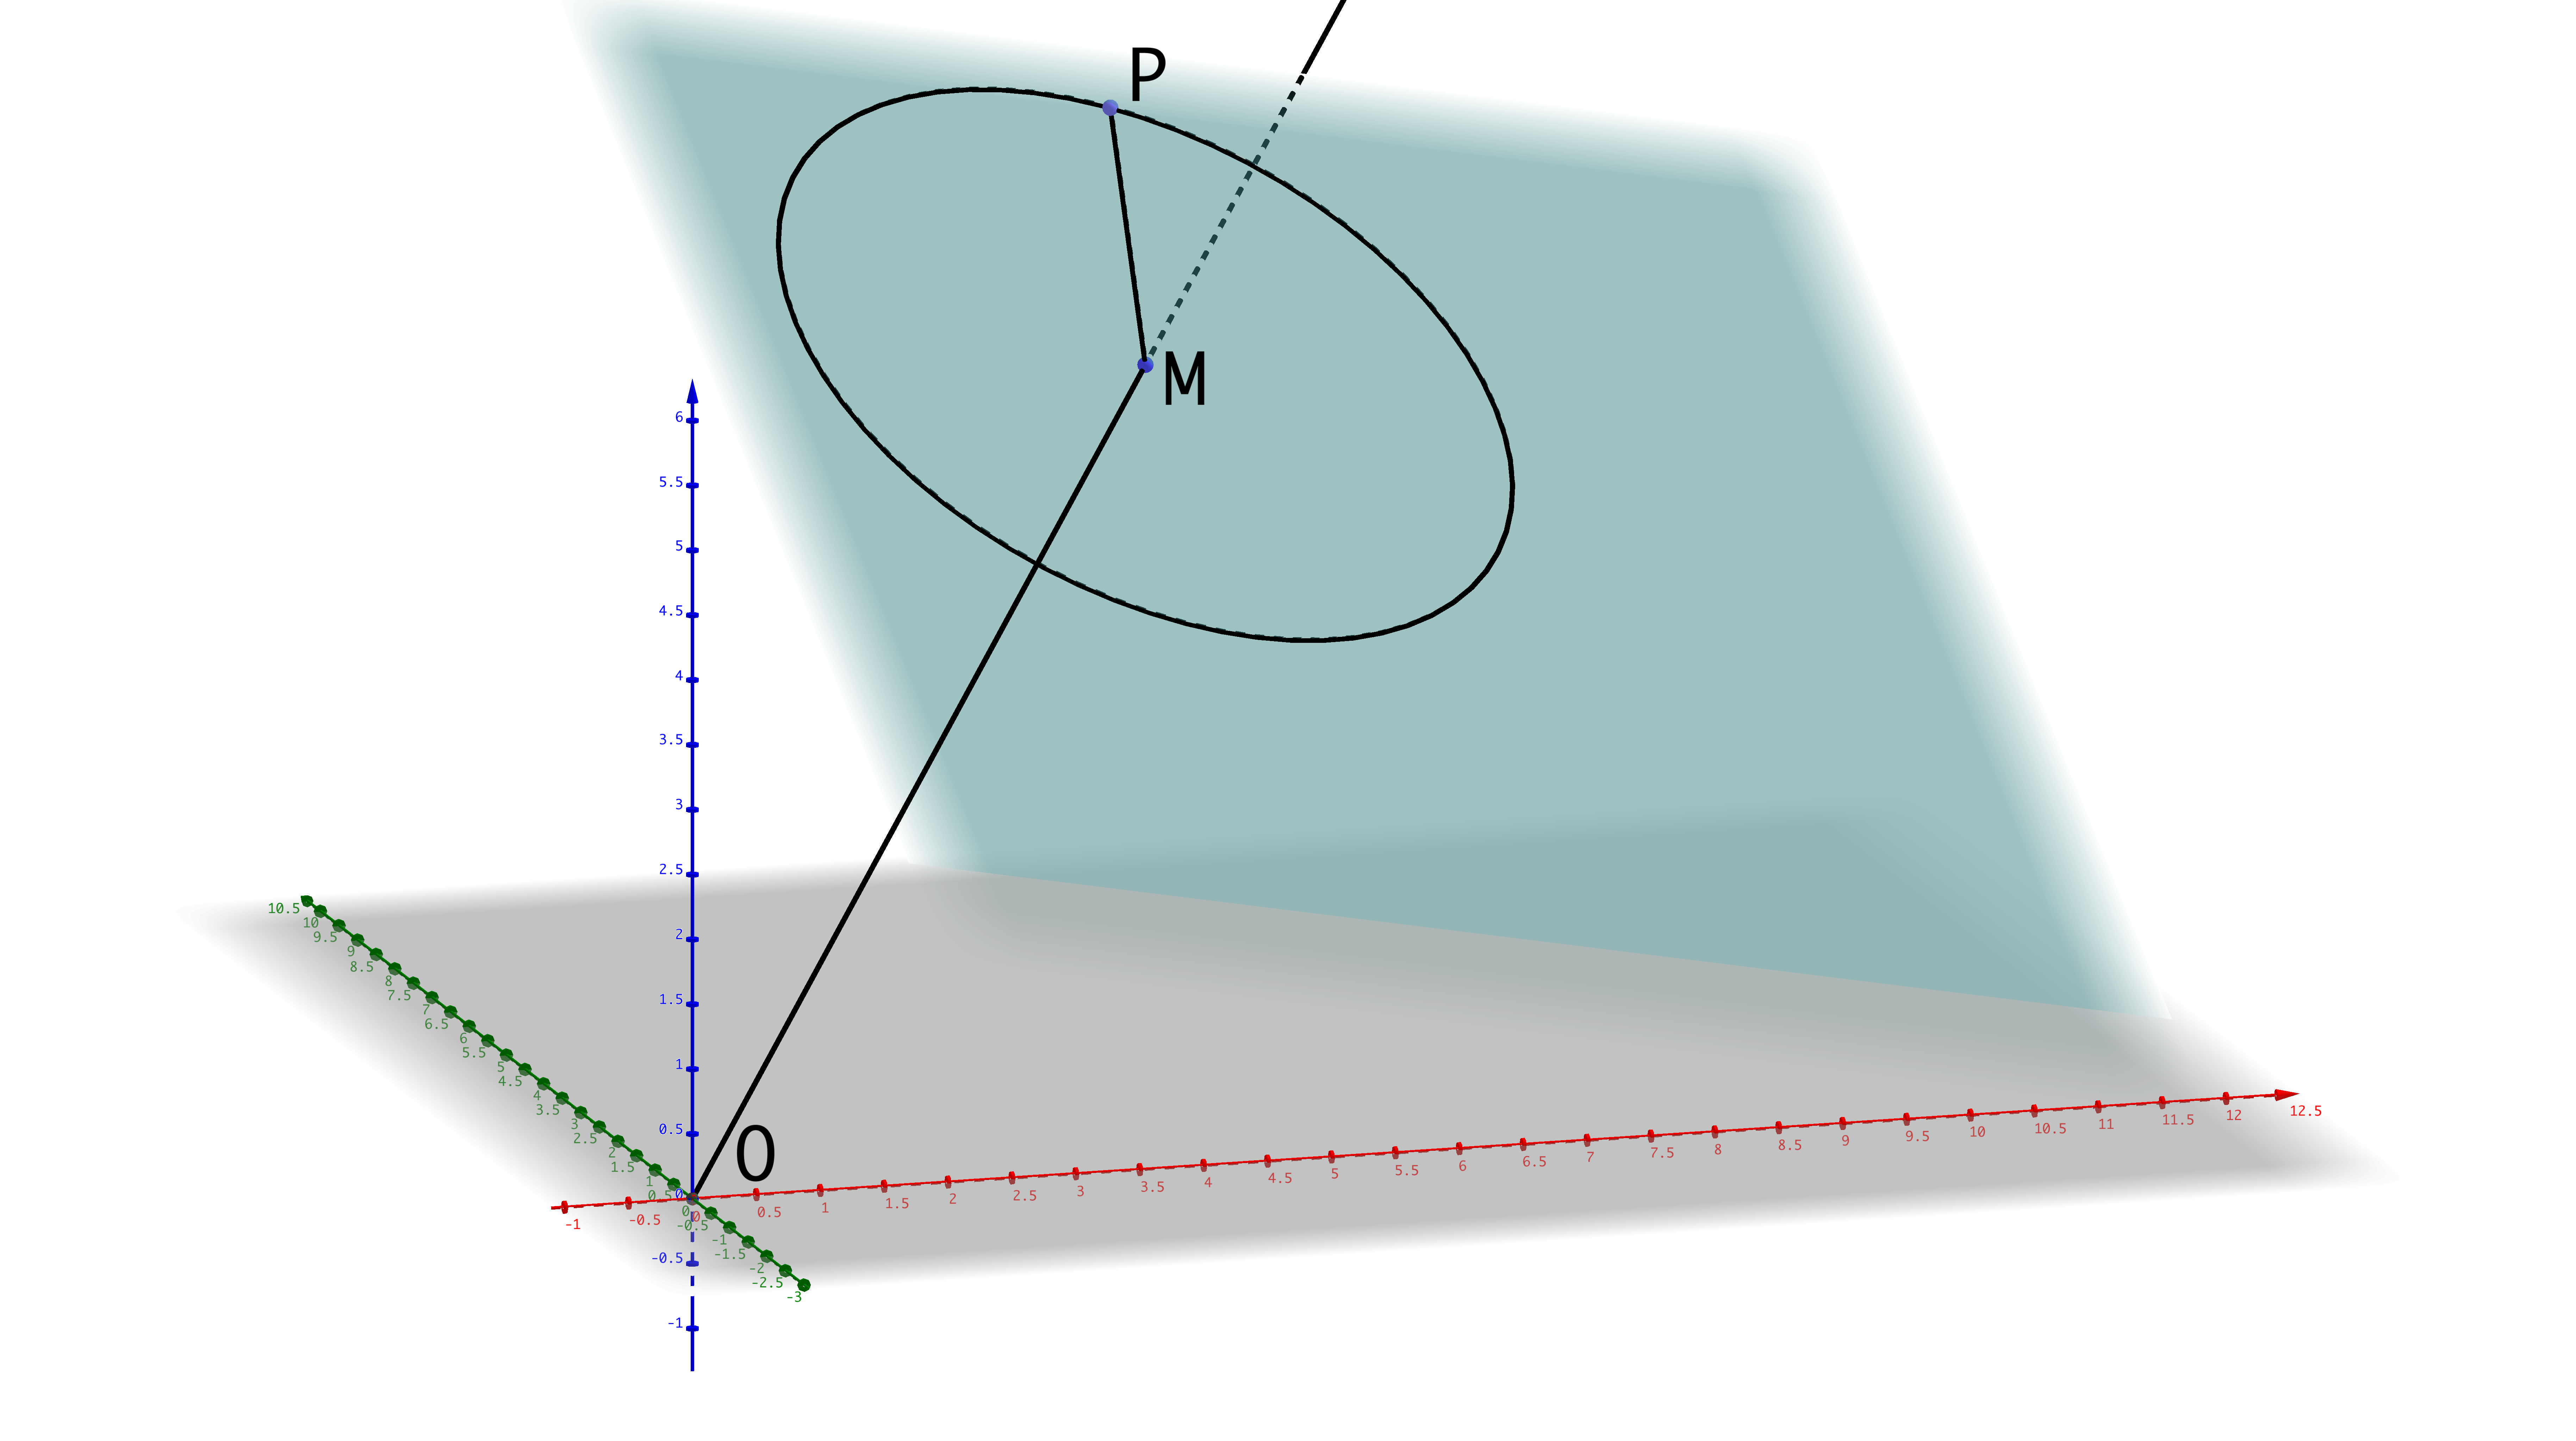
\includegraphics[width=10cm, height = 6cm]{figures/ndgeometry}
				\caption{一个三维空间中的例子}
			\end{figure}
	
			
			注意到 $OM$ 和 $P$ 所在超平面正交, 所以$\Delta \xi$ 和 $\Delta \eta$ 的变化是相互独立的. 它们对于体积的贡献也是独立的. 于是, 集合 \ref{ndgeometry} 所在的体积元体积为:
			
			\begin{equation}
				c \eta_0^{n-2} \Delta \xi_0 \Delta \eta_0
			\end{equation}
			其中 $c$ 是一个常数. 
			
			而样本的密度在这个体积元中几乎是一个常数, 为:
			
			\begin{equation}
				\begin{aligned}[]
					c \cdot \exp\left(- \frac{1}{2\sigma^2} \sum_{i=1}^n x_i^2\right) & =
					c \cdot \exp\left(- \frac{1}{2\sigma^2}(n\bar{x}^2 + \sum_{i=1}^n(x_i -\bar{x})^2)\right) \\
					& = c \cdot \exp\left(-\frac{1}{2\sigma^2} \xi_0^2\right) \cdot \exp\left(-\frac{1}{2\sigma^2} \eta_0^2\right)
				\end{aligned}
			\end{equation}
			
			这个式子和上面的体积元的表达式结合起来, 我们就可以得到元概率的表达式:
			
			\begin{equation}
				c \cdot \exp \left(-\frac{1}{2\sigma^2} \xi_0^2\right) \Delta \xi_0 \cdot \eta_0^{n-2} \exp\left(-\frac{1}{2\sigma^2} \eta_0^2\right) \Delta \eta_0
			\end{equation}
			
			这一举证明了 $\bar{x}$ 和 $s$ 的独立性.
			
			这个是一个比较有趣的地方, 对于 $t$ 分布的推导我们只有这个部分没有学习. 根据前文所述的证明梗概, 读者可以自行还原出 $t$ 分布的证明出来.


%\include{body/simplefigure}
%\include{body/simpletable}
%\include{body/simpleequation}
%\include{body/simplereference}


%参考文献
\defaultfont
\bibliographystyle{GBT7714-2005NLang-HIT}
\addcontentsline{toc}{chapter}{参考文献}      % 参考文献加入到中文目录
\addcontentsline{toe}{chapter}{\bfseries  References} % 参考文献加入到英文目录
\addtolength{\bibsep}{-0.8em}
\nocite{*}  %若将此命令屏蔽掉,则未引用的文献不会出现在文后的参考文献列表中。
\bibliography{reference}

\ifNeedAppendix
	% -*-coding: utf-8 -*-

\defaultfont
\appendix
%
%%%%%%%%%%%%%%%%%%%%%%%%%%%%%%%%%%%%%%%%%%%%%%%%%%%%%%%%%%
%\BiAppChapter{带章节的附录}{Full Appendix}%
%完整的附录内容,包含章节,公式,图表等
%
%%%%%%%%%%%%%%%%%%%%%%%%%%%%%%%%%%%%%%%%%%%%%%%%%%%%%%%%%%
%\BiSection{附录节的内容}{Section in Appendix}
%这是附录的节的内容
%
%附录中图的示例:
%\begin{figure}[htbp]
%\centering
%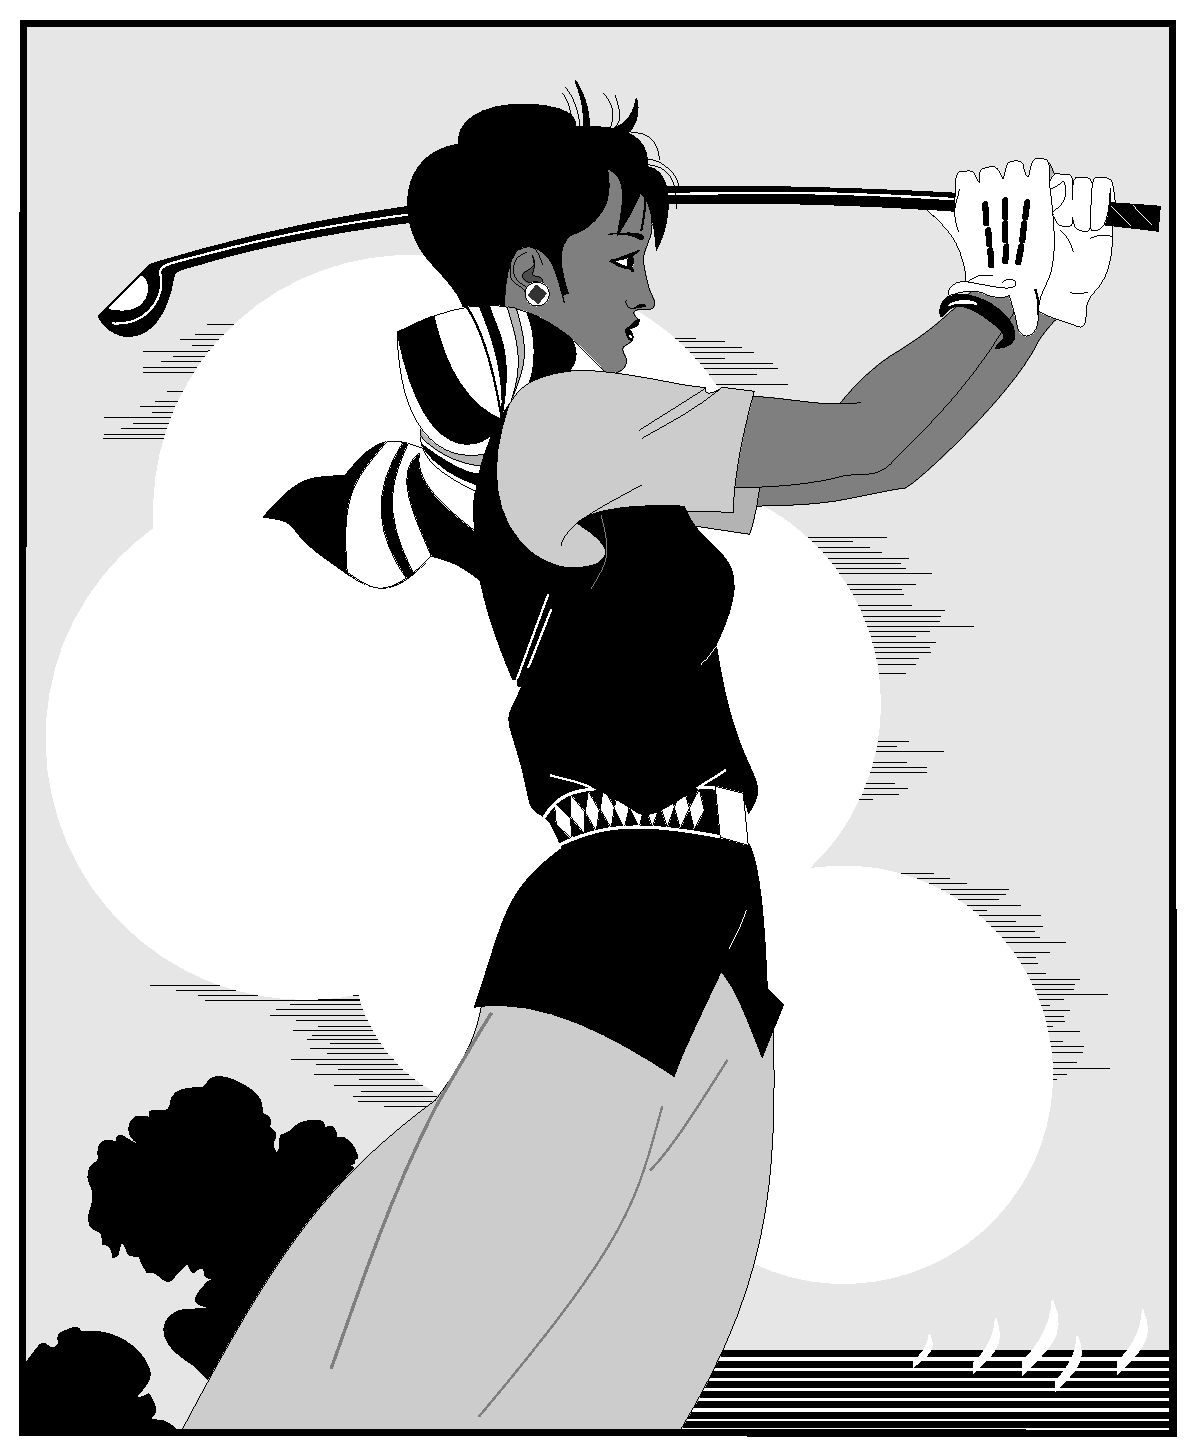
\includegraphics[width = 0.4\textwidth]{golfer}
%\bicaption[golfer5]{}{打高尔夫球的人}{Fig.$\!$}{The person playing golf}\vspace{-1em}
%\end{figure}
%
%附录中公式的示例:
%\begin{align}
%a & = b \times c \\
%E & = m c^2
%\end{align}
%
%%\BiAppChapter{附录二}{appendix 2}
%%\BiAppChapter{附录三}{appendix 3}

\chapter{}

\section{关于}    % 附录
	% !Mode:: "TeX:UTF-8" 

\defaultfont
\BiAppendixChapter{攻读\cxuewei 学位期间发表的论文及其他成果} {Papers
published in the period of PH.D. education}
\setlength{\parindent}{0em}
\textbf{(一)发表的学术论文}
\begin{publist}
\item	XXX,XXX. Static Oxidation Model of Al-Mg/C Dissipation Thermal Protection Materials[J]. Rare Metal Materials and Engineering, 2010, 39(Suppl. 1): 520-524.(SCI~收录,IDS号为~669JS,IF=0.16)
\item XXX,XXX. 精密超声振动切削单晶铜的计算机仿真研究[J]. 系统仿真学报,2007,19(4):738-741,753.(EI~收录号:20071310514841)
\item XXX,XXX. 局部多孔质气体静压轴向轴承静态特性的数值求解[J]. 摩擦学学报,2007(1):68-72.(EI~收录号:20071510544816)
\item XXX,XXX. 硬脆光学晶体材料超精密切削理论研究综述[J]. 机械工程学报,2003,39(8):15-22.(EI~收录号:2004088028875)
\item XXX,XXX. 基于遗传算法的超精密切削加工表面粗糙度预测模型的参数辨识以及切削参数优化[J]. 机械工程学报,2005,41(11):158-162.(EI~收录号:2006039650087)
\item XXX,XXX. Discrete Sliding Mode Cintrok with Fuzzy Adaptive Reaching Law on 6-PEES Parallel Robot[C]. Intelligent System Design and Applications, Jinan, 2006: 649-652.(EI~收录号:20073210746529)
\end{publist}

\textbf{(二)申请及已获得的专利(无专利时此项不必列出)}
\begin{publist}
\item XXX,XXX. 一种温热外敷药制备方案:中国,88105607.3[P]. 1989-07-26.
\end{publist}

\textbf{(三)参与的科研项目及获奖情况}
\begin{publist}
\item	XXX,XXX. XX~气体静压轴承技术研究, XX~省自然科学基金项目.课题编号:XXXX.
\item XXX,XXX. XX~静载下预应力混凝土房屋结构设计统一理论. 黑江省科学技术二等奖, 2007.
\end{publist}
\vfill
\hangafter=1\hangindent=2em\noindent

\setlength{\parindent}{2em}
    % 所发文章
	\ifxueweibachelor
  		% !Mode:: "TeX:UTF-8" 

\BiAppendixChapter{哈尔滨工业大学本科毕业设计(论文)原创性声明}{Statement of copyright and Letter of authorization}

本人郑重声明:在哈尔滨工业大学攻读学士学位期间,所提交的毕业设计(论文)《\chinesethesistitle》,是本人在导师指导下独立进行研究工作所取得的成果。对本文的研究工作做出重要贡献的个人和集体,均已在文中以明确方式注明,其它未注明部分不包含他人已发表或撰写过的研究成果,不存在购买、由他人代写、剽窃和伪造数据等作假行为。

本人愿为此声明承担法律责任。

\vspace{\baselineskip}
\hspace{6em}作者签名:\hfill 日期:\hspace{2.5em}年\hspace{1.5em}月\hspace{1.5em}日
 % 本科蛋疼承诺
	\else
	  % !Mode:: "TeX:UTF-8" 

\BiAppendixChapter{哈尔滨工业大学学位论文原创性声明及使用授权说明}{Statement of copyright and Letter of authorization}
\vspace{\baselineskip}
\begin{center}\hei\xiaosan{学位论文原创性声明}\end{center}
\vspace{1em}

本人郑重声明:此处所提交的学位论文《\chinesethesistitle》,是本人在导师指导下,在哈尔滨工业大学攻读学位期间独立进行研究工作所取得的成果。据本人所知,论文中除已注明部分外不包含他人已发表或撰写过的研究成果。对本文的研究工作做出重要贡献的个人和集体,均已在文中以明确方式注明。本声明的法律结果将完全由本人承担。

\vspace{\baselineskip}
\hspace{6em}作者签名:\hfill 日期:\hspace{2.5em}年\hspace{1.5em}月\hspace{1.5em}日

\vspace{3\baselineskip}
\begin{center}\hei\xiaosan{学位论文使用授权说明}\end{center}
\vspace{1em}

本人完全了解哈尔滨工业大学关于保存、使用学位论文的规定,即:

(1)已获学位的研究生必须按学校规定提交学位论文;(2)学校可以采用影印、缩印或其他复制手段保存研究生上交的学位论文;(3)为教学和科研目的,学校可以将学位论文作为资料在图书馆及校园网上提供目录检索与阅览服务;(4)根据相关要求,向国家图书馆报送学位论文。

保密论文在解密后遵守此规定。
\vspace{\baselineskip}

本人保证遵守上述规定。

\vspace{2\baselineskip}
\hspace{6em}作者签名:\hfill 日期:\hspace{2.5em}年\hspace{1.5em}月\hspace{1.5em}日

\vspace{2\baselineskip}
\hspace{6em}导师签名:\hfill 日期:\hspace{2.5em}年\hspace{1.5em}月\hspace{1.5em}日 % 硕博承诺
	\fi   
	% !Mode:: "TeX:UTF-8" 

\BiAppendixChapter{致\quad 谢}{Acknowledgements}

衷心感谢导师~XXX~教授对本人的精心指导。他的言传身教将使我终生受益。

感谢~XXX~教授,以及实验室全体老师和同窗们的热情帮助和支持!

本课题承蒙~XXXX~基金资助,特此致谢。

…
% 致谢

	\ifxueweidoctor
		% !Mode:: "TeX:UTF-8" 

\defaultfont

\BiAppendixChapter{个人简历}{Resume}

XXXX~年~XX~月~XX~日出生于~XXXX。

XXXX~年~XX~月考入~XX~大学~XX~院(系)XX~专业,XXXX~年~XX~月本科毕业并获得~XX~学学士学位。

XXXX~年~XX~月------XXXX~年~XX~月在~XX~大学~XX~院(系)XX~学科学习并获得~XX~学硕士学位。

XXXX~年~XX~月------XXXX~年~XX~月在~XX~大学~XX~院(系)XX~学科学习并获得~XX~学博士学位。

获奖情况:如获三好学生、优秀团干部、X~奖学金等(不含科研学术获奖)。

工作经历:

\vspace{3em}\noindent
\textbf{( 除全日制硕士生以外,其余学生均应增列此项。个人简历一般应包含教育经历和工作经历。)}          % 博士学位论文有个人简介
	\fi
\fi

\clearpage

\end{document}